% Licencia y derechos: consulte ../../LICENSE-CC-BY-4.0.
% Las figuras y demás materiales de terceros pueden tener derechos separados y deben identificarse.

\chapter{Amplificadores de varias etapas} %p70

En el capítulo anterior, se demostró una relación inversa entre ganancia y ancho de banda cuando se analizó el amplificador emisor común para altas frecuencias. Esto es indicativo de los límites en los posibles alcances con una sola etapa. En el presente capítulo se estudiará configuraciones de varias etapas que permitirán mejorar las características del conjunto, como por ejemplo, aumentar la impedancia de entrada de un amplificador u obtener una mayor frecuencia de corte alta para una ganancia dada. También se verá como puede acoplarse etapas directamente para así amplificar corriente continua. En este aspecto saldrá a relucir la configuración diferencial, la cual se analizará a fondo. Finalmente se presentarán amplificadores comerciales fabricados como circuitos integrados que también amplifican en corriente continua.

\section{Sistemas de varias etapas: Generalidades} %p70

En la Figura \ref{fig:multietapas_sistema-cascada} se plantea un sistema de varias etapas en cascada. Las características de mayor interés de un sistema son la ganancia de voltaje, \( A_V \), la ganancia de corriente, \( A_I \), la resistencia de entrada \( R_i \), la resistencia de salida \( R_o \) y el rango de frecuencias de operación del sistema.

\begin{figure}[h]
	\centering
	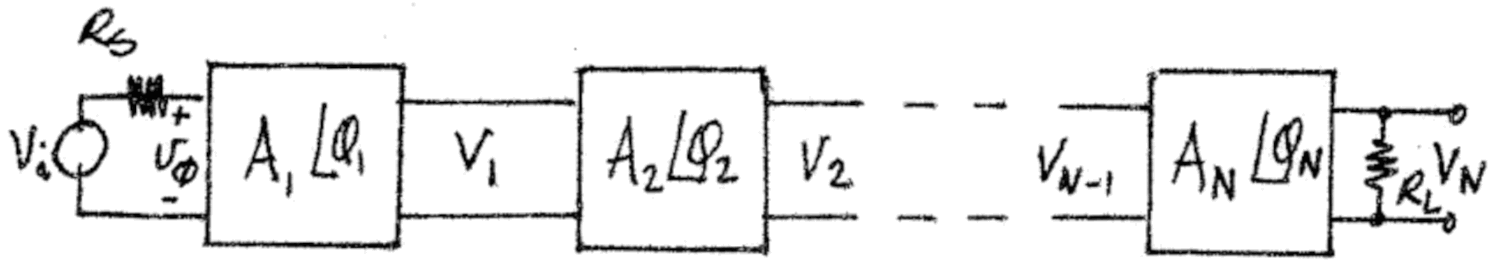
\includegraphics[width=0.8\linewidth]{_fig/multietapas_sistema-cascada.png}
	\caption{Sistema de varias Etapas en Cascada}
	\label{fig:multietapas_sistema-cascada}
\end{figure}

En el sistema:

\begin{equation}
	\frac{V_o}{V_s} (\omega) = \frac{R_i}{(R_{i1} + R_s)} = A_{\phi} (\omega) \angle \phi_{\phi} (\omega)
\end{equation}

\begin{equation}
	\frac{V_N}{V_{N-1}} (\omega) = A_N (\omega) \angle \phi_N (\omega)
\end{equation}

Después los totales vienen dados por:

\begin{equation}
	\left| \frac{V_N}{V_s} \right| = \left| \frac{V_N}{V_{N-1}} \right| \left| \frac{V_{N-1}}{V_{N-2}} \right| \cdots \left| \frac{V_i}{V_{\phi}} \right| \left| \frac{V_{\phi}}{V_s} \right| = A_N A_{N-1} \cdots A_1 A_{\phi}
\end{equation}

\begin{equation}
	\angle \frac{V_N}{V_s} = \phi_N + \phi_{N-1} + \cdots + \phi_1 + \phi_0
\end{equation}

La ganancia en forma logarítmica queda como una suma:

\begin{equation}
	\log \left| \frac{V_N}{V_s} \right| = \log A_N + \log A_{N-1} + \cdots + \log A_1 + \log A_{\phi}
\end{equation}

Para un amplificador con flujo de señal unilateral, se plantea un modelo general, como se muestra en la Figura \ref{fig:multietapas_rep-amp}.

\begin{figure}[h]
	\centering
	\subfloat[Modelo general]
	{
		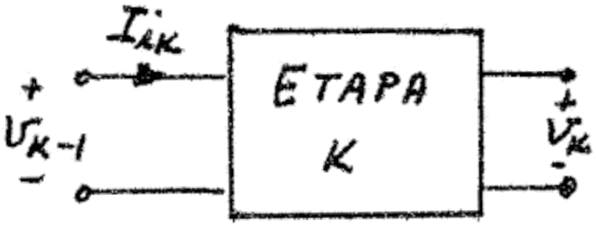
\includegraphics[width=0.32\linewidth]{_fig/multietapas_rep-amp_modelo-general.png}
		\label{fig:multietapas_rep-amp_modelo-general}
	}
	\subfloat[Basado en fuente de voltaje controlado]
	{
		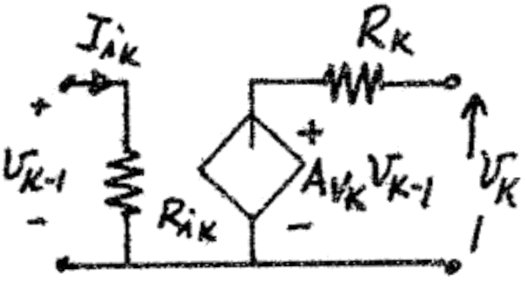
\includegraphics[width=0.32\linewidth]{_fig/multietapas_rep-amp_voltaje-controlado.png}
		\label{fig:multietapas_rep-amp_voltaje-controlado}
	}
	\subfloat[Basado en fuente de corriente controlado]
	{
		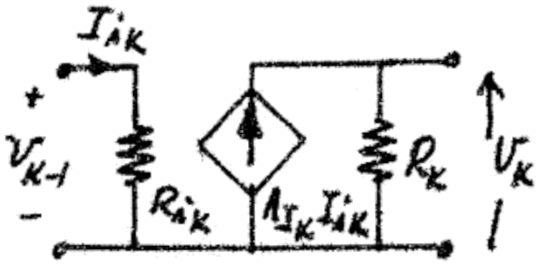
\includegraphics[width=0.32\linewidth]{_fig/multietapas_rep-amp_corriente-controlado.png}
		\label{fig:multietapas_rep-amp_corriente-controlado}
	}
	\caption{Representaciones de Amplificadores}
	\label{fig:multietapas_rep-amp}
\end{figure}

En la Figura \ref{fig:multietapas_rep-amp}, \( A_{Ik} \) es la ganancia de corriente de la etapa con la salida en corto circuito, y \( A_{Vk} \) es la ganancia de tensión de la etapa sin carga. Se consigue:

\begin{equation}
	V_k = A_{Ik} I_{ik} R_k
\end{equation}

también

\begin{equation}
	I_{ik} = V_{k-1} / R_{ik}
\end{equation}

y la relación entre ganancia de voltaje y corriente viene dada por:

\begin{equation}
	A_{Vk} = \frac{V_k}{V_{k-1}} = A_{Ik} \frac{R_k}{R_{ik}}
\end{equation}

Al anexar otra etapa, vea la Figura \ref{fig:multietapas_conexion-otra-etapa}, se cae la ganancia inter-etapas.

\begin{equation}
	A_K = \frac{V_K}{V_{K-1}} = \frac{R_{i(K+1)}}{R_{i(K+1)} + R_K} A_{VK}
\end{equation}

ademas

\begin{equation}
	A_K' = \frac{I_{i(K+1)}}{I_{ik}} = A_{IK} \frac{R_K}{R_K + R_{i(K+1)}}
\end{equation}

\begin{figure}[h]
	\centering
	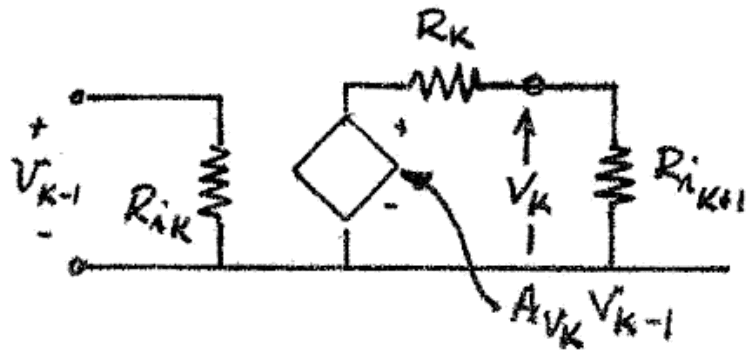
\includegraphics[width=0.8\linewidth]{_fig/multietapas_conexion-otra-etapa.png}
	\caption{Conexión de otra etapa}
	\label{fig:multietapas_conexion-otra-etapa}
\end{figure}

La ganancia de voltaje total, \( A_{VT} \), viene dada por

\begin{equation}
	A_{VT} = \frac{A_{IT} R_L}{R_S + R_{i1}}
\end{equation}

donde \( A_{IT} \) es la ganancia de corriente total y viene dada por

\begin{equation}
	A_{IT} = A_{I1} A_{I2} \cdots A_{IN}'
\end{equation}

En general la resistencia de salida del conjunto es la resistencia de salida de la última etapa, y la resistencia de entrada es la de la primera etapa.

\section{La configuración Darlington} %p72

La Configuración Darlington, que se muestra en la Figura \ref{fig:multietapas_conf-darlington}, está formado por dos transistores que conforman un super-transistor, es decir representan un dispositivo de tres contactos cuya ganancia de corriente es aproximadamente el cuadrado de la de un solo transistor.

\begin{figure}[h]
	\centering
	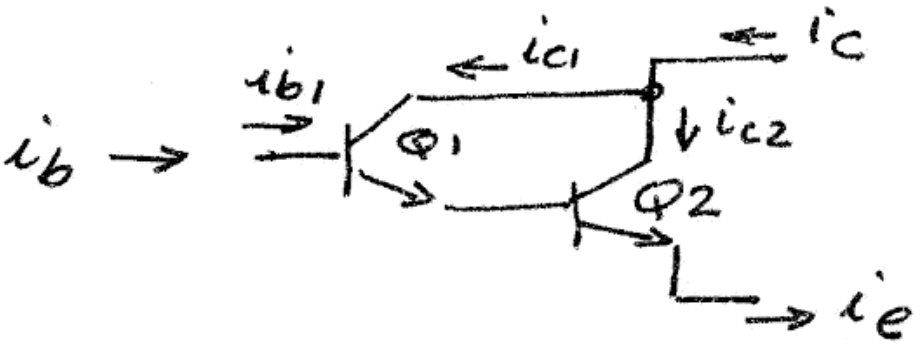
\includegraphics[width=0.8\linewidth]{_fig/multietapas_conf-darlington.png}
	\caption{Configuración Darlington}
	\label{fig:multietapas_conf-darlington}
\end{figure}

Partiendo de este diagrama se obtienen las siguientes ecuaciones:

\[ i_c = i_{c1} + i_{c2} \]
\[ i_{c1} = \beta_1 i_{b1} \]
\[ i_{b2} = (\beta_1 + 1) i_{b1} \]
\[ i_c = \beta_1 i_{b1} + \beta_2 i_{b2} = \beta_1 i_{b1} + \beta_2 (\beta_1 + 1) i_{b1} \]

para eventualmente llegar a:

\begin{equation}
	i_c = [\beta_1 + \beta_1 \beta_2 + \beta_2] i_{b1} = (\beta+2)\beta i_b
\end{equation}

De aquí se desprende que la relación entre la corriente de "colector" y la corriente de base es \( \beta + 2 \) veces mayor que esta relación para una sola etapa. Si para una etapa la \( \beta \) es 100, con la configuración Darlington, la "\( \beta \)" es mas de 10.000.

\subsection{Ejemplo 1} \label{multietapas_ejm1}
Para el circuito de la Figura \ref{fig:multietapas_conf-darlington_colector-comun}, determine a) la corriente de base de entrada en continua, y b) la resistencia de entrada. Utilice \( \beta = 100 \) para los transistores.

\begin{figure}[h]
	\centering
	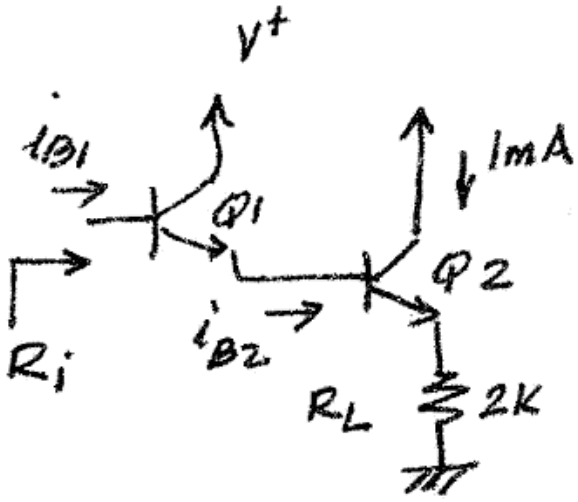
\includegraphics[width=0.5\linewidth]{_fig/multietapas_conf-darlington_colector-comun.png}
	\caption{Configuración Darlington como Colector Común}
	\label{fig:multietapas_conf-darlington_colector-comun}
\end{figure}

\textbf{Solución.}

Dado que la corriente por \( R_L = 1 mA\) , entonces la corriente de base de Q2 \( I_{BQ2} = 10 \mu A\) , y la corriente de base de Q1 \( I_{BQ1} \approx 0.1 \mu A\) . Por lo tanto,

\[ r_{\pi 1} = \frac{\beta}{g_{m1}} = \frac{100 \times 25 mV}{100 \mu A} = 250 k\Omega \]

\[ r_{\pi 2} = 2.5 k\Omega \]

y

\[ R_L = r_{\Pi 1} + (\beta_1 +1) \left[ (r_{\Pi 2} + (\beta_1 +1) R_L \right] = 20.9 M\Omega \]

En el Ejemplo \ref{multietapas_ejm1}, se obtiene un valor elevadísimo para la resistencia de entrada. De la misma forma, se reduce la resistencia de salida, y en líneas generales se logra aumentar tremendamente la ganancia de corriente de la configuración respecto a la de un solo transistor.			

\section{La configuracion Cascodo} %p74

La configuración Cascode, que se muestra en la Figura \ref{fig:multietapas_cascodo}, es particularmente recomendable para obtener un ancho de banda amplio. Como se demostrará más adelante, esta configuración tiene en común con la configuración EC las expresiones para las ganancias de voltaje y corriente, y las resistencias de entrada y salida. Se diferencia en que el ancho de banda es mayor, la capacitancia de entrada es menor y la ganancia inversa de voltaje, \( h \), es mucho menor.

En la Figura \ref{fig:multietapas_cascodo_frecuencias-medias} se muestra el circuito para frecuencias medias; se consiguen las relaciones de las ecuaciones \ref{multietapas_cascodo_frecuencias-medias-equ1} y \ref{multietapas_cascodo_frecuencias-medias-equ2}.

\begin{figure}[h]
	\centering
	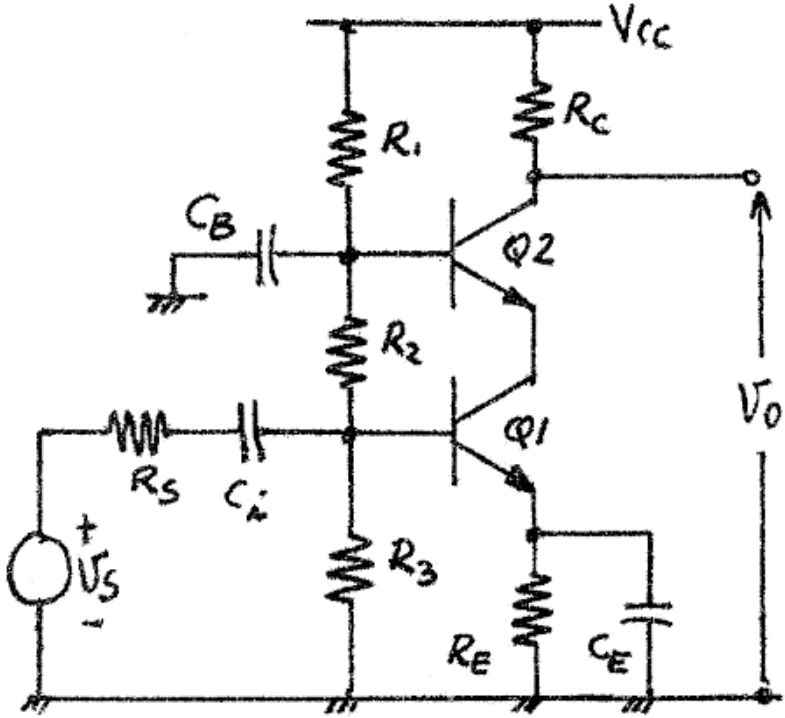
\includegraphics[width=0.5\linewidth]{_fig/multietapas_cascodo.png}
	\caption{El Cascodo}
	\label{fig:multietapas_cascodo}
\end{figure}

\begin{equation} \label{multietapas_cascodo_frecuencias-medias-equ1}
	\frac{I_o}{I_2} = \frac{\beta}{\beta +1} \approx 1 \quad \frac{I_2}{I_1} = -\beta \quad \Rightarrow \quad \frac{I_o}{I_1} \approx -\beta
\end{equation}

y

\begin{equation} \label{multietapas_cascodo_frecuencias-medias-equ2}
	\frac{V_o}{V_i} = \frac{I_o R_C}{I_i r_{\Pi}} = -\beta \frac{R_C}{r_{\Pi}} = -g_m R_C
\end{equation}

\begin{figure}[h]
	\centering
	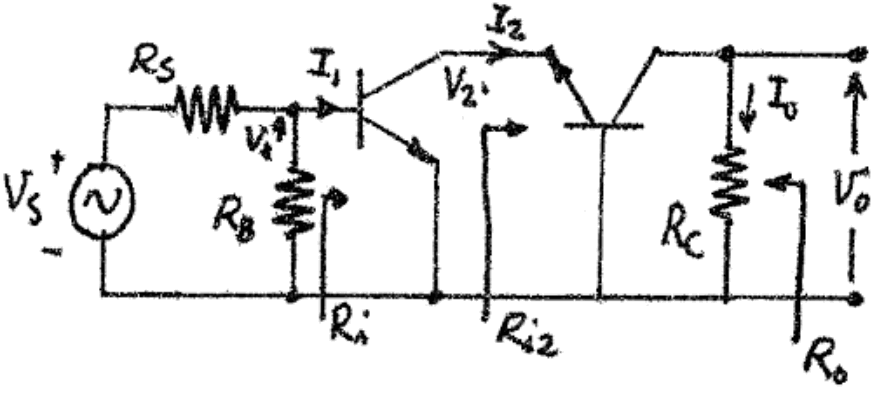
\includegraphics[width=0.5\linewidth]{_fig/multietapas_cascodo_frecuencias-medias.png}
	\caption{El Cascodo, frecuencias medias}
	\label{fig:multietapas_cascodo_frecuencias-medias}
\end{figure}

Además, $R_i = r_{\Pi}$ y $R_o = R_C$. En comparación con una configuración emisor común, se observa que la configuración cascode tiene las mismas expresiones para las ganancias de voltaje y corriente, y las resistencias de entrada y salida.

Determinación de $w_{gB}$: $C_j$ y $C_B$ tendrán expresiones para sus polos que se consiguieron en la configuración Emisor Común. En la Figura \ref{fig:multietapas_cascodo_hallar-wcb} se muestra el circuito apto para hallar el polo debido a $C_B$.

\begin{figure}[h]
	\centering
	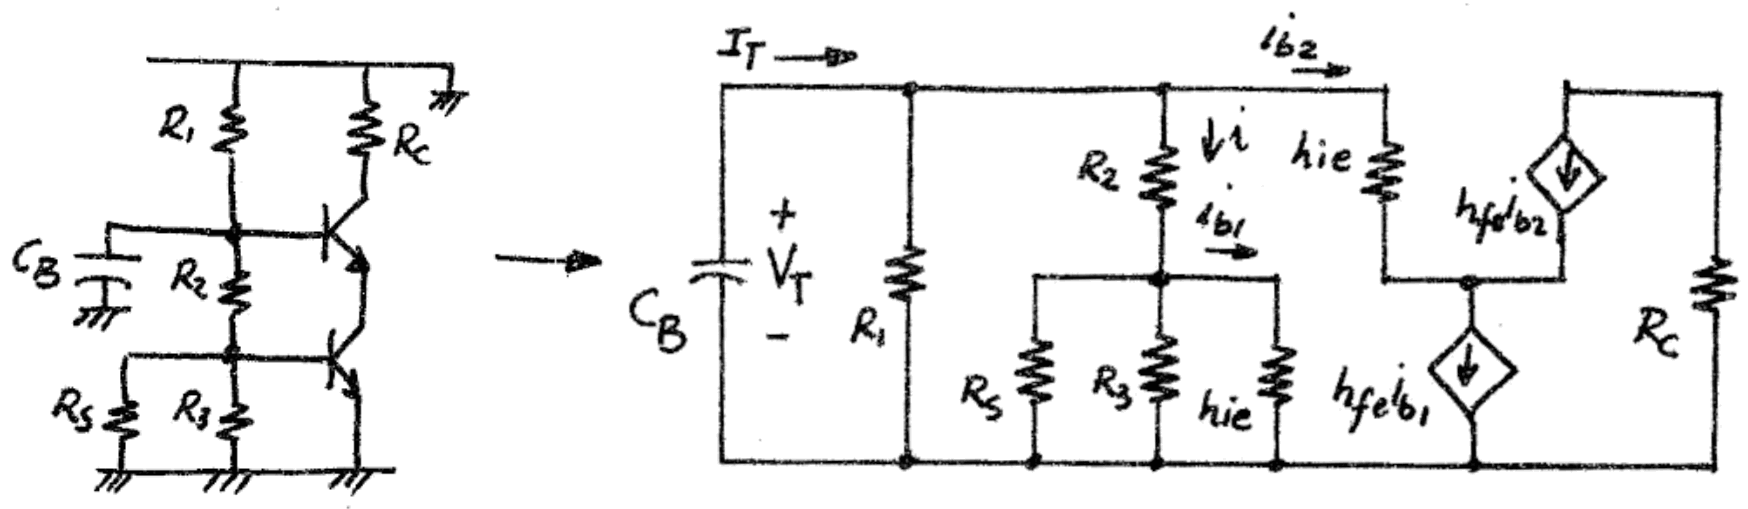
\includegraphics[width=0.8\linewidth]{_fig/multietapas_cascodo_hallar-wcb.png}
	\caption{Circuito para hallar $w_{CB}$}
	\label{fig:multietapas_cascodo_hallar-wcb}
\end{figure}

De él se desarrolla lo siguiente:

\[
I_T = \frac{V_T}{R_1} + \frac{V_T}{R_2 + R_3 \parallel R_s \parallel h_{ie}} + i_{b2}
\]

\[
i_{b1} = \frac{R_s \parallel R_3}{R_s \parallel R_3 + h_{ie}} i = \frac{R_s \parallel R_3}{R_s \parallel R_3 + h_{ie}} \cdot \frac{V_T}{R_2 + R_s \parallel R_3 \parallel h_{ie}}
\]

\[
i_{b2} = \frac{h_{fe1}}{h_{fe2} +1} i_{b1} = \frac{h_{fe1}}{h_{fe2} +1} \cdot \frac{R_s \parallel R_3}{R_s \parallel R_3 + h_{ie}} \cdot \frac{V_T}{R_2 + R_s \parallel R_3 \parallel h_{ie}}
\]

\[
R_{Th} = \frac{V_T}{I_T} = \frac{1}{\frac{1}{R_1} + \frac{1}{R_2 + \beta_3 h_{fe} h_{ie}} (1+ \frac{h_{fe}}{h_{fe} +1} \frac{R_s \parallel R_3}{R_s \parallel R_3 + h_{ie}})}
\]

Después:

\[
w_B = w_{Ci} + w_{CE} + w_{CB}
\]

Para altas frecuencias, los condensadores $C_i$, $C_E$ y $C_B$ se consideran cortocircuitos y se plantea el circuito equivalente, en donde se utiliza el modelo híbrido para los transistores, como se muestra en la Figura \ref{fig:multietapas_cascodo_frecuencias-altas}.

\begin{figure}[h]
	\centering
	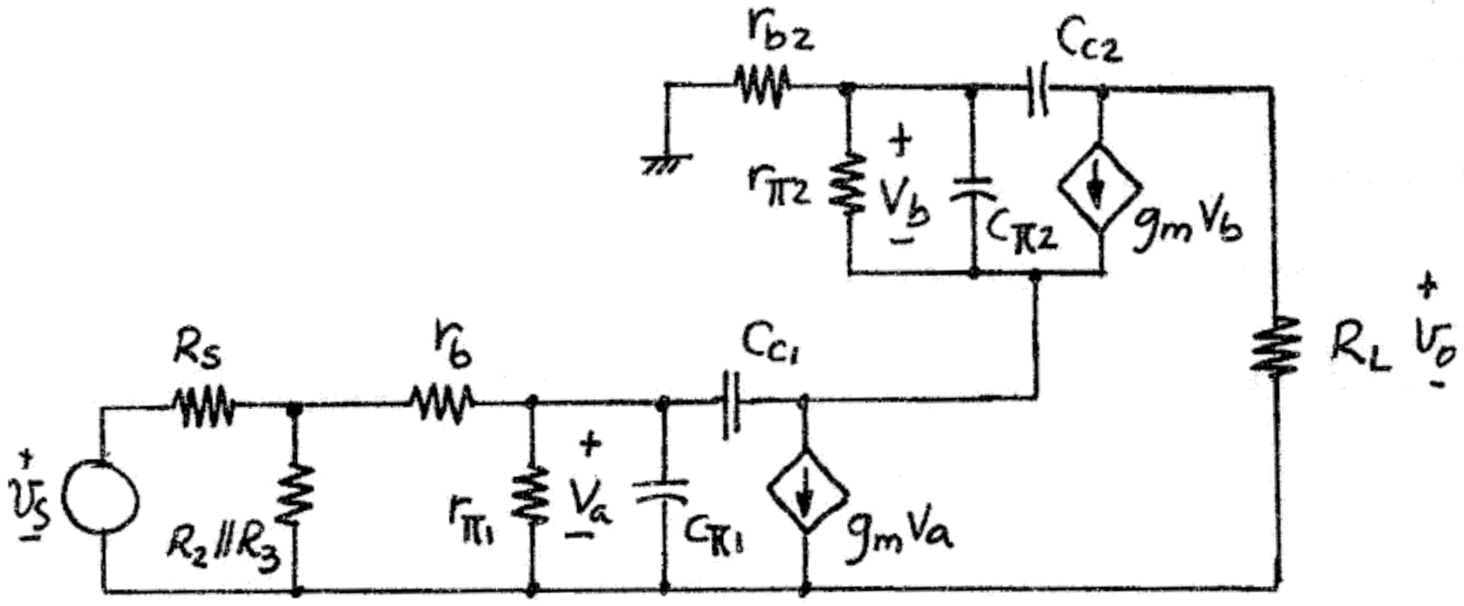
\includegraphics[width=0.8\linewidth]{_fig/multietapas_cascodo_frecuencias-altas.png}
	\caption{Modelo del Cascode para Altas Frecuencias}
	\label{fig:multietapas_cascodo_frecuencias-altas}
\end{figure}

Para hallar la constante de tiempo de $C_{T1}$, se reduce el circuito de la Figura \ref{fig:multietapas_cascodo_frecuencias-altas}, a lo que se ve en la Figura 2.10a.

Entonces:

\begin{equation} \label{multietapas_cascodo_constantes-de-tiempo-eq}
	\tau_{CT1} = C_{T1} \cdot (r_{\pi} \parallel r_6')
\end{equation}

Para \( C_C \) queda:

\begin{equation} \label{multietapas_cascodo_constantes-de-tiempo-eq-cc}
	\tau_{CC1} = C_{C1} \left[ (r_{\pi} \parallel r_6') + R_1 + g_m R_L (r_{\pi} \parallel r_6') \right]
\end{equation}

\begin{figure}[h]
	\centering
	\subfloat[Para \( C_{\pi 1} \)]
	{
		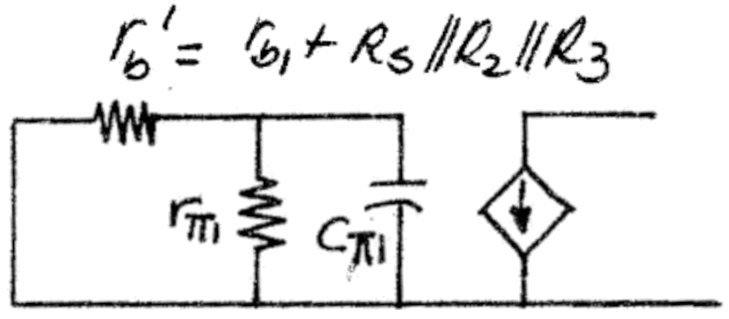
\includegraphics[width=0.32\linewidth]{_fig/multietapas_cascodo_constantes-de-tiempo-a.png}
		\label{fig:multietapas_cascodo_constantes-de-tiempo-a}
	}
	\subfloat[]
	{
		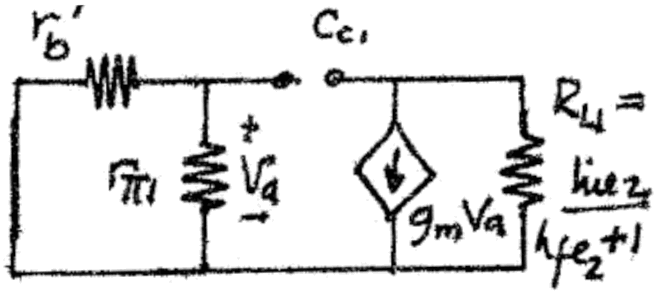
\includegraphics[width=0.32\linewidth]{_fig/multietapas_cascodo_constantes-de-tiempo-b.png}
		\label{fig:multietapas_cascodo_constantes-de-tiempo-b}
	}
	\subfloat[]
	{
		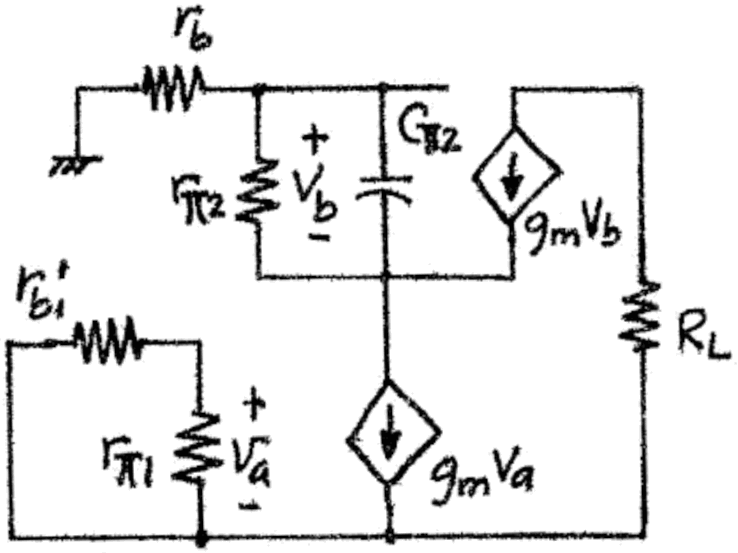
\includegraphics[width=0.32\linewidth]{_fig/multietapas_cascodo_constantes-de-tiempo-c.png}
		\label{figmultietapas_cascodo_constantes-de-tiempo-c}
	}
	\subfloat[]
	{
		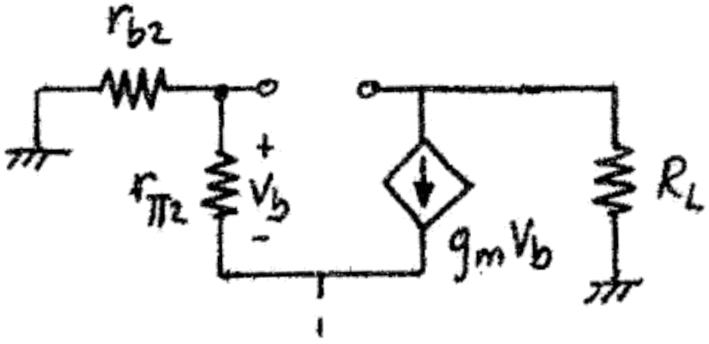
\includegraphics[width=0.32\linewidth]{_fig/multietapas_cascodo_constantes-de-tiempo-d.png}
		\label{fig:multietapas_cascodo_constantes-de-tiempo-d}
	}
	\caption{Circuitos para hallar las constantes de tiempo}
	\label{fig:multietapas_cascodo_constantes-de-tiempo}
\end{figure}

donde \( R_{L1} \) es la resistencia de carga de \( Q_1 \), es decir, la \( R_i \) de entrada de \( Q_2 \), \( R_{L1} = \frac{r_{\pi 2}}{\beta + 1} \)

Para \( C_{\pi 2} \), se hace notar que \( V_a = 0 \), con lo que se elimina el circuito de abajo.

Luego:

\[
I_T = \frac{V_T}{r_{\pi 2}} + g_{m2} V_b = V_T \left(\frac{1}{r_{\pi 2}} + g_{m2} \right)
\]

\[
R_T = \frac{r_{\pi 2}}{(1 + g_{m2} r_{\pi 2})} = \frac{r_{\pi 2}}{(\beta + 1)}
\]

\begin{equation} \label{multietapas_cascodo_eq1}
	\tau_{C\pi 2} = C_{\pi 2} \cdot \frac{r_{\pi 2}}{(\beta + 1)}
\end{equation}

Para \( C_{c2} \), se observa que en el nodo emisor de \( Q_2 \) puede plantearse así:

\[
\frac{V_b}{r_{\pi}} + g_m V_b = 0
\]

De donde concluimos que \( V_b = 0 \), y no circula corriente por esas ramas.

Entonces:

\begin{equation} \label{multietapas_cascodo_eq2}
	R_{Th} = r_{b2} + R_L, \quad \tau_{Cc2} = C_{c2} (r_{b2} + R_L)
\end{equation}

Luego, la frecuencia de corte alta viene dada por:

\[
\omega_H \approx \frac{1}{(C_{\pi 1} + C_{cc1} + \tau_{C\pi 2} + \tau_{Cc2})}
\]

\subsection{Ejemplo 2}
En el circuito de la Figura 2.11 se han polarizado ambos transistores con el mismo punto de operación: \( I_C = 2.1 mA \), \( V_{CE} = 4.5 V \). De donde: \( g_m = 0.081 \), \( \beta = 132 \), \( r_b = 60\), \( r_{\pi} = 1640 \), \( C_c = 2.2 pF \), \( C_{\pi} = 48 pF \).

\begin{figure}[h]
	\centering
	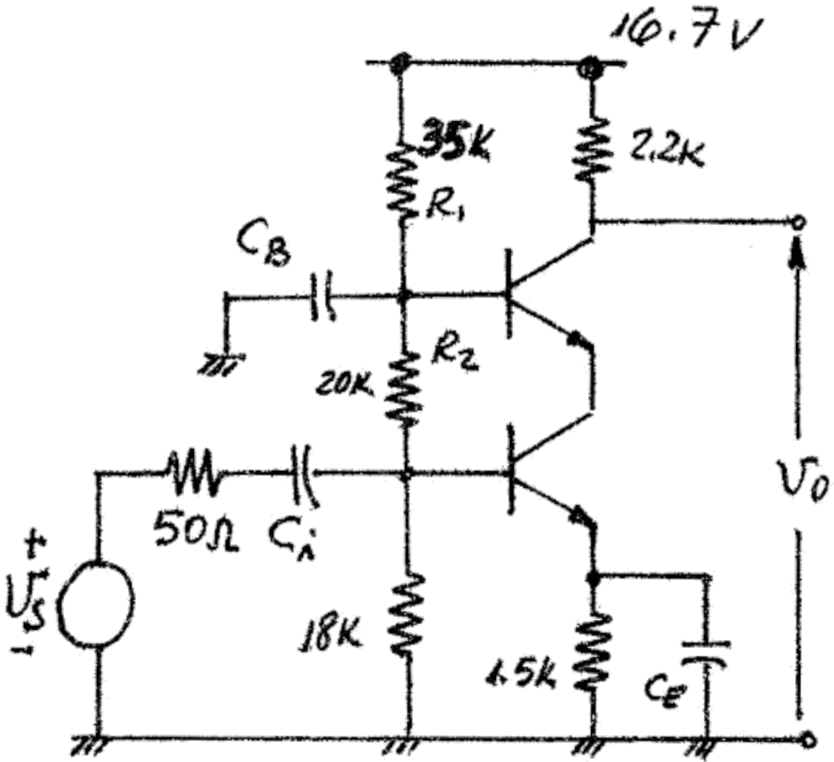
\includegraphics[width=0.8\linewidth]{_fig/multietapas_cascodo_ejemplo.png}
	\caption{Circuito de Ejemplo}
	\label{fig:multietapas_cascodo_ejemplo}
\end{figure}

Entonces, de la ecuación \ref{multietapas_cascodo_constantes-de-tiempo-eq}:

\[
\tau_{C\pi 1} = 48 \times 10^{-12} \left( 1640 \parallel ((60 + 20K) \parallel 18K \parallel 50) \right)
\]

\[
\tau_{C\pi 1} = 4.94 \times 10^{-9}
\]

de la ecuación \ref{multietapas_cascodo_constantes-de-tiempo-eq-cc}

\[
\tau_{Cc1} = 2.2 \times 10^{-12} \left(103 + \frac{1700}{133} + 0.081 \times 103 \times 1700 \right)
\]

\[
\tau_{Cc1} = 0.235 \times 10^{-9}
\]

De la ecuación \ref{multietapas_cascodo_eq1}:

\[
\tau_{C\pi 2} = 48 \times 10^{-12} \left( \frac{1640}{133} \right) = 0.68 \times 10^{-9}
\]

De la ecuación \ref{multietapas_cascodo_eq2}:

\[
\tau_{Cc2} = 2.2 \times 10^{-12} \left( 60 + 2200 \right) = 4.97 \times 10^{-9}
\]

Luego:

\[
\sum \tau = (4.94 + 0.23 + 0.68 + 4.97) \times 10^{-9} = 10.7 \times 10^{-9}
\]

y 

\[
\omega_H = \frac{1}{2\sum \tau} = \frac{1}{10.7 \times 10^{-9}} = 93.1 \times 10^6 rad/s
\]

\[
f_H = 14.8 MHz
\]

Esta cifra se puede comparar con el resultado del Ejemplo \ref{respfreq_ejm6} de un circuito emisor común con la misma ganancia, y se nota que se ha aumentado la frecuencia de corte alta por un factor de aproximadamente \( 7 \).

Además, en el circuito emisor común, se calcula el valor de la capacitancia de entrada, como:

\[
C_{entcascodo} = C_{\pi} + (1 + g_m R_L) C_c = 48 + (1 + 0.081 \times 2.2K) 2.2 = 442 pF
\]

En cambio, con los mismos datos para la configuración cascode, el valor de la capacitancia de entrada viene dado por:

\[
C_{entcascodo} = C_{\pi} + \left( 1 + g_m \frac{r_{\pi}}{\beta + 1} \right) C_{c2}
\]

\[
C_{entcascodo} = 48 + \left( 1 + 0.081 \times \frac{1700}{133} \right) 2.2 = 52.5 pF
\]

Es decir, se ha reducido la capacitancia de entrada por un factor de \( 12 \).

Finalmente, se hace notar que por medio del Método de Superposición, se puede determinar cuál de las constantes de tiempo es la más dominante, y por lo tanto la que se tiene que reducir primero si se quiere aumentar la frecuencia de corte alta.

\section{Acoplamiento directo de circuitos} %p79

Con los métodos sencillos dados, se puede analizar una configuración a fin de conseguir la frecuencia de corte deseada de alta o de baja. Para aumentar la frecuencia de corte alta, se hace necesario reducir el valor de las constantes de tiempo. Para disminuir la frecuencia de corte baja, se procura reducir el valor de los polos de los condensadores, lo cual se consigue directamente al aumentar el valor de los condensadores. Sin embargo, esta puede ser una medida costosa ya que los condensadores de valor mayor de $1 \mu F$, tienen un costo proporcional a su capacitancia y a su voltaje máximo.

Una alternativa para reducir la frecuencia de corte baja consiste en eliminar condensadores; por ejemplo, si se acopla dos etapas directamente se elimina el condensador de acople. El diseño de circuitos electrónicos sin condensadores es de interés particular para los circuitos integrados ya que las capacitancias que se pueden crear con esta técnica son muy pequeñas y ocupan mucho espacio.

Se comenzará a plantear las consideraciones a tomar en cuenta para eliminar condensadores con el ejemplo de una cascada de etapas emisor común.

\begin{figure}[h]
	\centering
	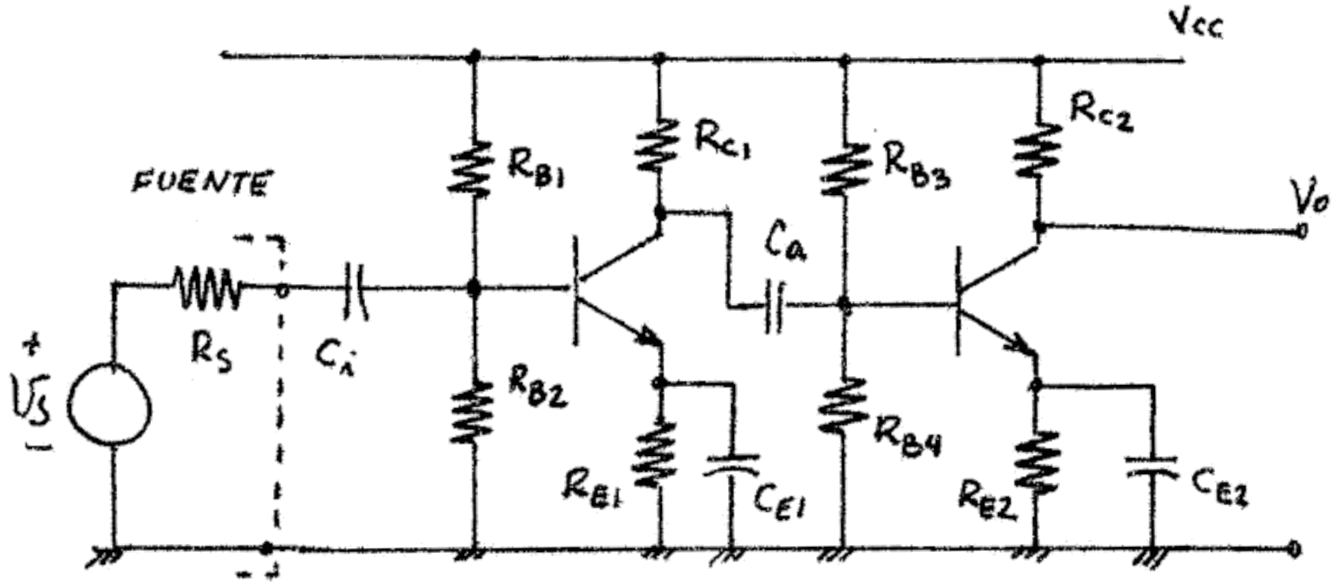
\includegraphics[width=0.8\linewidth]{_fig/multietapas_cascada-etapa-ec.png}
	\caption{Cascada de etapas EC}
	\label{fig:multietapas_cascada-etapa-ec}
\end{figure}

En la Figura \ref{fig:multietapas_cascada-etapa-ec}, se puede eliminar a $C_A$, y de paso a $R_{B3}$ y $R_{B4}$, para llegar a la configuración de la Figura \ref{fig:multietapas_cascada-etapa-ec-sin-ca}.

\begin{figure}[h]
	\centering
	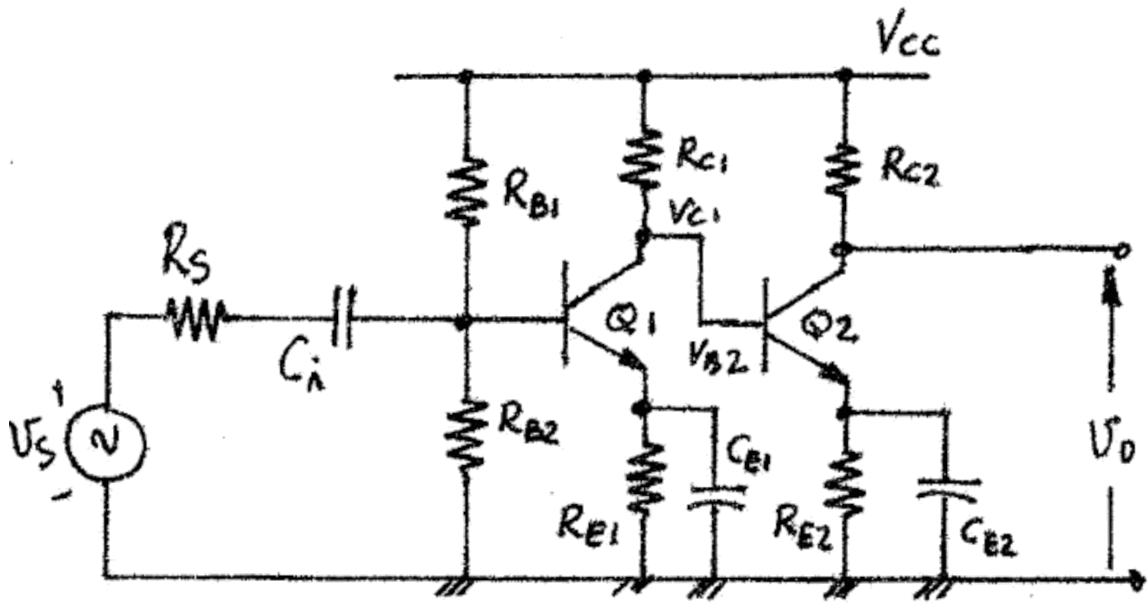
\includegraphics[width=0.8\linewidth]{_fig/multietapas_cascada-etapa-ec-sin-ca.png}
	\caption{Cascada de etapas EC sin \( C_a \)}
	\label{fig:multietapas_cascada-etapa-ec-sin-ca}
\end{figure}

Se puede conectar el colector de $Q_1$ directamente a la base de $Q_2$ cuando el nivel de continua en estas dos puntos es el mismo.

\begin{figure}[h]
	\centering
	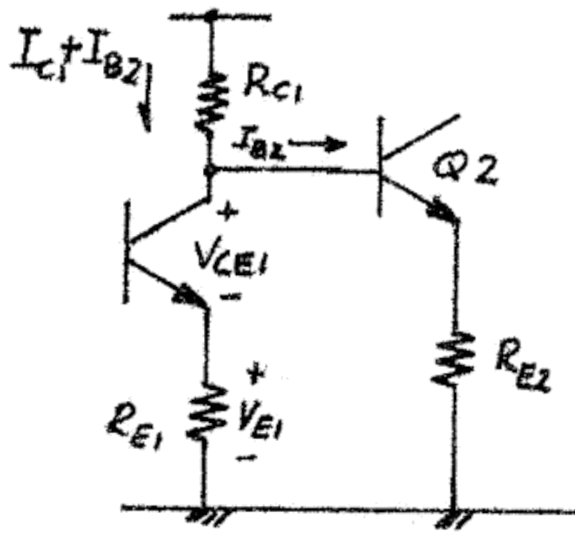
\includegraphics[width=0.8\linewidth]{_fig/multietapas_cascada-etapa-ec_pol-segunda-etapa.png}
	\caption{Cascada EC, polarización segunda etapa}
	\label{fig:multietapas_cascada-etapa-ec_pol-segunda-etapa}
\end{figure}

Para este circuito, la polarización de la primera etapa queda igual. El circuito de polarización de la segunda etapa se muestra en la Figura \ref{fig:multietapas_cascada-etapa-ec_pol-segunda-etapa}. La corriente que pasa por $R_{C1}$ es $I_{C1} + I_{B2}$, $R_{E2}$ puede ser escogida para que se cumpla la condición necesaria de \( V_{C1} = V_{B2} \); se hace notar que la polarización de la segunda etapa está íntimamente relacionada con la polarización de la primera etapa. Es decir, queda:

\[
R_{E2} = \frac{V_{CC} - (I_{C1} + I_{B2})R_{C1} - V_{BE2}}{(\beta +1) I_{B2}}
\]

La misma idea se aplica a fin de eliminar $C_i$ a la entrada del amplificador; para acoplar la fuente directamente al amplificador tiene que existir el mismo nivel de continua en los puntos a conectar. En el caso general, la fuente de entrada tiene un nivel de continua igual a cero, por lo que se modifica el amplificador a fin de que también tenga un nivel de continua igual a cero en su entrada.

Se logra llevar la entrada a cero volt, y a la vez polarizar la junta BE del transistor de entrada, al utilizar una fuente de poder bipolar (positiva y negativa), como se muestra en la Figura \ref{fig:multietapas_cascada-etapa-ec_fuente-bipolar}.

\begin{figure}[h]
	\centering
	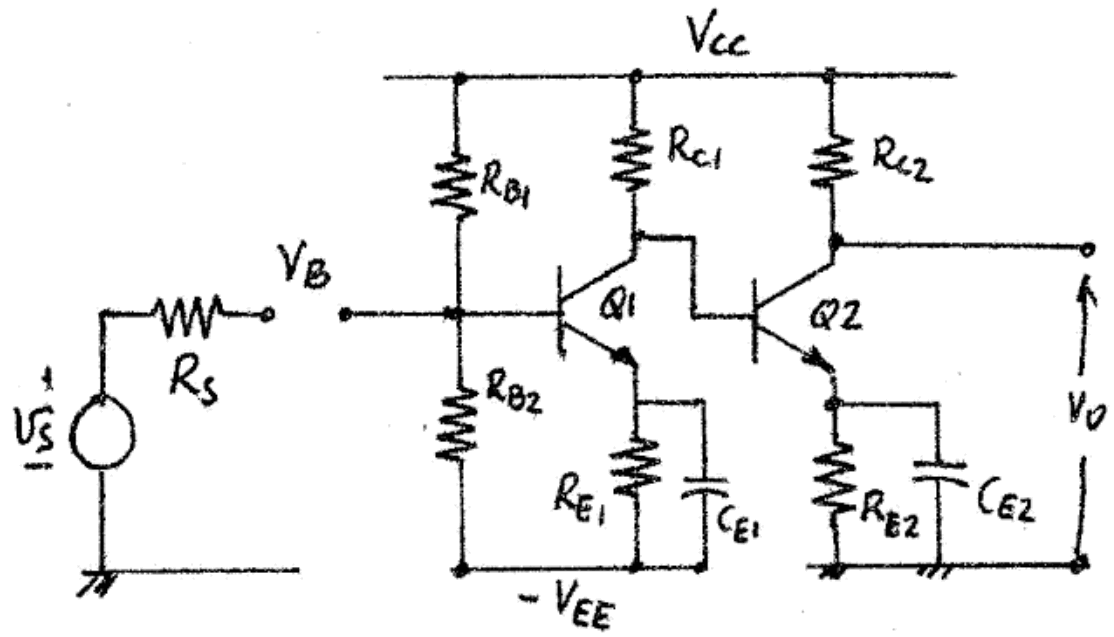
\includegraphics[width=0.8\linewidth]{_fig/multietapas_cascada-etapa-ec_fuente-bipolar.png}
	\caption{Cascada EC, con fuente bipolar}
	\label{fig:multietapas_cascada-etapa-ec_fuente-bipolar}
\end{figure}

Se ajusta los valores de $R_{B1}$ y $R_{B2}$ de modo que el nivel continuo de $V_B$ sea igual a 0. También se podría eliminar $R_{B1}$ y $R_{B2}$, y en tal caso, la corriente de base de polarización es suministrada por la fuente de entrada. Esto crea un pequeño nivel negativo $= -I_B R_S$, a la entrada del amplificador. Vea la Figura \ref{fig:multietapas_cascada-etapa-ec_sin-rb}.

\begin{figure}[h]
	\centering
	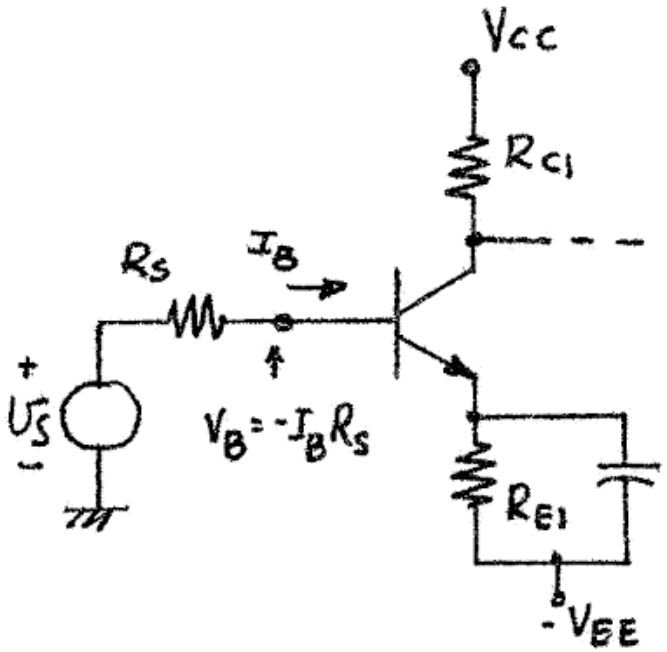
\includegraphics[width=0.8\linewidth]{_fig/multietapas_cascada-etapa-ec_sin-rb.png}
	\caption{Cascada EC, entrada sin \( R_B \)}
	\label{fig:multietapas_cascada-etapa-ec_sin-rb}
\end{figure}

Dado nuestro objetivo de un amplificador sin condensadores, aún nos quedan los de puenteo de emisor, $C_{E1}$ y $C_{E2}$ en la Figura \ref{fig:multietapas_cascada-etapa-ec_fuente-bipolar}. Veamos $C_E$ y $R_E$: $R_E$ le imprime una estabilidad térmica a la etapa, y a su vez, $C_E$ la puentea a frecuencias medias a fin de aumentar la ganancia del circuito. En la Figura \ref{fig:multietapas_amp-fuente-continua}, se plantean dos amplificadores de corriente continua. El de la Figura \ref{fig:multietapas_amp-fuente-continua_buena-ganancia} tiene buena ganancia pero mala estabilidad térmica. El de la Figura \ref{fig:multietapas_amp-fuente-continua_buena-estabilidad} tiene buena estabilidad térmica pero poca ganancia.

\begin{figure}[h]
	\centering
	\subfloat[Buena Ganancia]
	{
		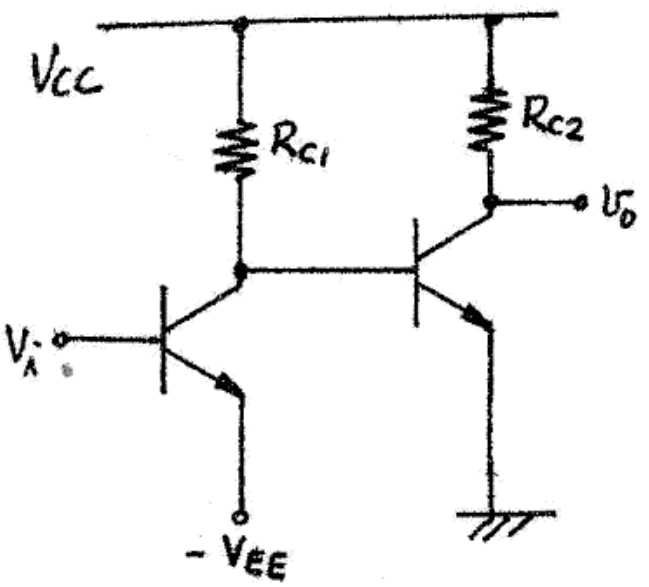
\includegraphics[width=0.46\linewidth]{_fig/multietapas_amp-fuente-continua_buena-ganancia.png}
		\label{fig:multietapas_amp-fuente-continua_buena-ganancia}
	}
	\subfloat[Buena Estabilidad Térmica]
	{
		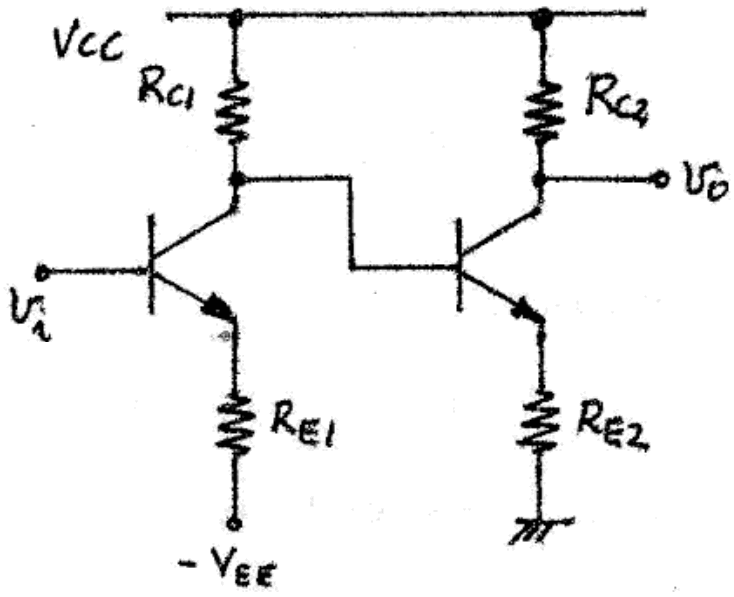
\includegraphics[width=0.46\linewidth]{_fig/multietapas_amp-fuente-continua_buena-estabilidad.png}
		\label{fig:multietapas_amp-fuente-continua_buena-estabilidad}
	}
	\caption{Amplificadores de corriente continua}
	\label{fig:multietapas_amp-fuente-continua}
\end{figure}

\section{La configuracion diferencial} %p83

La configuración que logra combinar una ganancia buena con una estabilidad térmica excelente es la configuración diferencial de la Figura \ref{fig:multietapas_conf-diferencial}. La resistencia de emisor es la que le proporciona su buena estabilidad térmica. A su vez, la cascada de transistores le proporciona una buena ganancia.

Antes de analizar en detalle esta configuración, vamos a presentar algunas características de la configuración diferencial general. Se hace notar que hay dos entradas y una salida sencilla, que se representa esquemáticamente en la Figura \ref{fig:multietapas_esquema-sistema-diferencial}. La diferencia entre las entradas se llama la entrada diferencial, $V_d$, donde:

\begin{equation}
	V_d = V_1 - V_2
\end{equation}

\begin{figure}[h]
	\centering
	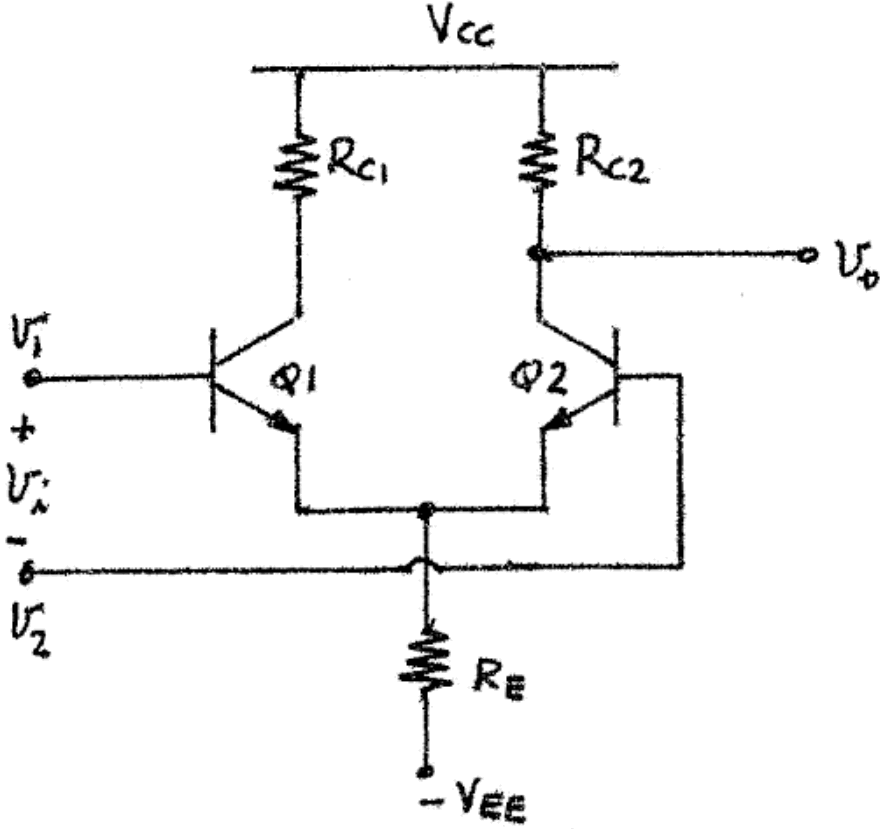
\includegraphics[width=0.6\linewidth]{_fig/multietapas_conf-diferencial.png}
	\caption{La configuración diferencial}
	\label{fig:multietapas_conf-diferencial}
\end{figure}

\begin{figure}[h]
	\centering
	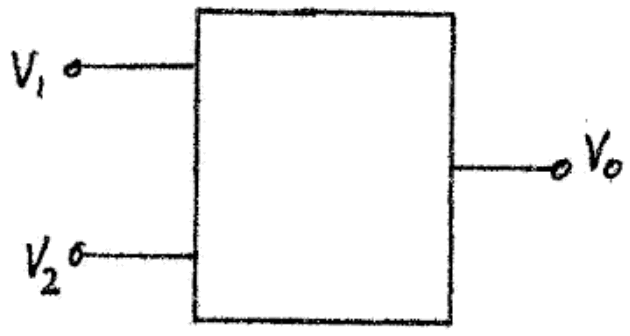
\includegraphics[width=0.4\linewidth]{_fig/multietapas_esquema-sistema-diferencial.png}
	\caption{Esquema de sistema diferencial}
	\label{fig:multietapas_esquema-sistema-diferencial}
\end{figure}

A su vez, las entradas tienen un componente común, que viene dado por el valor promedio de las entradas,

\begin{equation}
	V_c = (V_1 + V_2)/2
\end{equation}

Se tiene:

\begin{equation}
	V_o = A_1 V_1 + A_2 V_2
\end{equation}

donde

\begin{equation}
	A_1 = \frac{V_o}{V_1} \quad \text{con } V_2 = 0
\end{equation}

\begin{equation}
	A_2 = \frac{V_o}{V_2} \quad \text{con } V_1 = 0
\end{equation}

Alternativamente, podemos expresar a $V_o$ en función de la señal diferencial de entrada, y la componente común. Entonces:

\begin{equation}
	V_o = A_d V_d + A_c V_c
\end{equation}

Si se expresan las señales $V_1$ y $V_1$ en función de las señales $V_d$ y $V_c$ se obtiene:

\begin{equation}
	V_1 = V_c + \frac{V_d}{2}
\end{equation}

\begin{equation}
	V_2 = V_c - \frac{V_d}{2}
\end{equation}

Se puede relacionar las ganancias $A_1$ y $A_2$ con las ganancias de $A_d$ y $A_c$ y se obtiene:

\begin{equation} \label{multietapas_conf-diff_ac}
	A_c = A1 + A2
\end{equation}

\begin{equation} \label{multietapas_conf-diff_ad}
	A_d = \frac{A1 + A2}{2}
\end{equation}

\subsection{Ejemplo 3}

\textbf{Demuestre las relaciones de las Ecuaciones \ref{multietapas_conf-diff_ac} y \ref{multietapas_conf-diff_ad}.}

En los llamados Amplificadores Diferenciales se busca resaltar la ganancia diferencial frente a la ganancia de modo común. Un criterio de calidad para un amplificador5 diferencial es la relación entre la ganancia de modo diferencial y la de modo común, conocida como la relación de rechazo de modo común, que generalmente se expresa en $dB$.

\begin{equation}
	\text{CMRR} = 20 log | \frac{A_d}{A_c} | 
\end{equation}

Frecuentemente, los amplificadores diferenciales están diseñados para servir como amplificadores de corriente continua. El nivel de continua que se puede aplicar simultaneamente a ambas entradas está limitado y se conoce como el \textbf{Rango de Modo Común}. Si se aplica un nivel común fuera de éste rango, el circuito deja de trabajar como amplificador lineal, y eventualmente se puede dañar.

\subsection{Circuito simétrico con salida sencilla entrada diferencial} %p85

Vamos a analizar al circuito diferencial con el cual comenzamos esta sección, la Figura \ref{fig:multietapas_conf-diferencial}. Encontraremos las relaciones salida/entrada de dos modos: por medio del modelo de pequeña señal, y utilizando el Teorema de Bisección que describiremos después.

Más adelante veremos que la configuración diferencial tiene tanto una zona lineal de operación como una zona no lineal. En la Figura \ref{fig:multietapas_superposicion-ac_conf-diferencial} se plantea el modelo de pequeña señal y al mismo tiempo se aplica el Teorema de Superposición para encontrar la salida \( V_o \) en función de las dos entradas \( V_1 \) y \( V_2 \), es decir, 

\[
A_1 = \frac{V_o}{V_1}, \quad A_2 = \frac{V_o}{V_2}.
\]

El Teorema de Superposición es aplicable solo si el circuito trabaja en forma lineal.

\begin{figure}[h]
	\centering
	\subfloat[Para hallar \( A_1 \)]
	{
		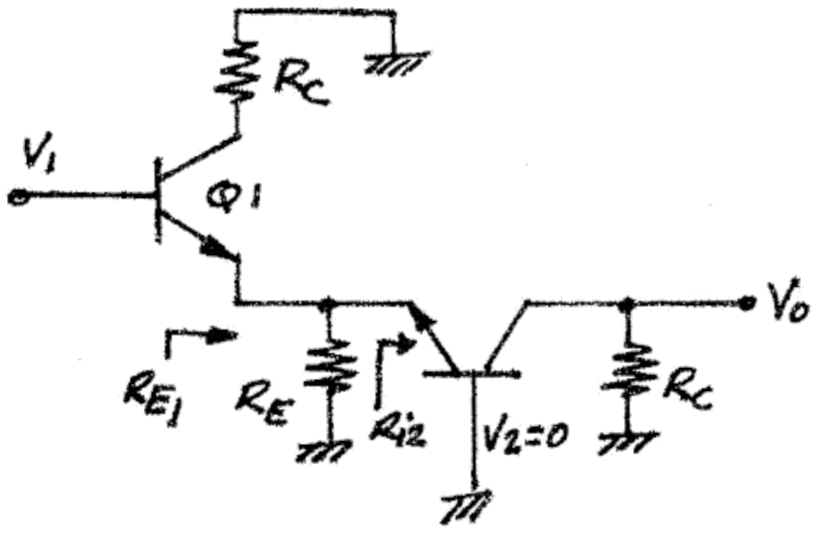
\includegraphics[width=0.46\linewidth]{_fig/multietapas_superposicion-ac_conf-diferencial-a1.png}
		\label{fig:multietapas_superposicion-ac_conf-diferencial-a1}
	}
	\subfloat[Para hallar \( A_2 \)]
	{
		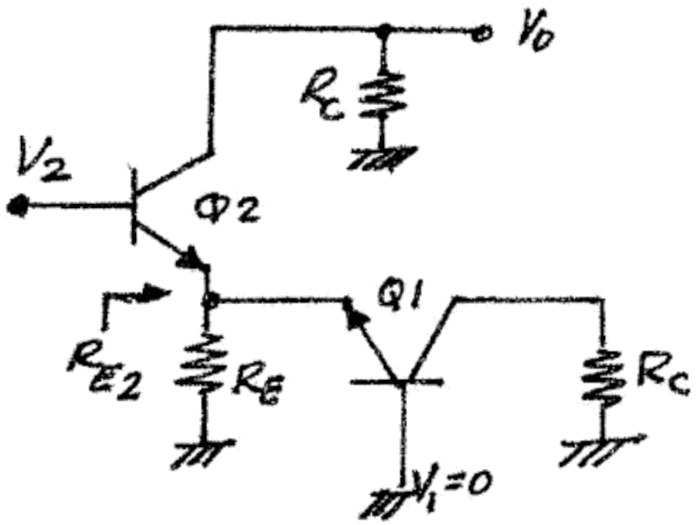
\includegraphics[width=0.46\linewidth]{_fig/multietapas_superposicion-ac_conf-diferencial-a2.png}
		\label{fig:multietapas_superposicion-ac_conf-diferencial-a2}
	}
	\caption{Teorema de Superposición aplicado en AC a la Configuración Diferencial}
	\label{fig:multietapas_superposicion-ac_conf-diferencial}
\end{figure}

En la Figura \ref{fig:multietapas_superposicion-ac_conf-diferencial-a1}, \( \frac{V_o}{V_1} = \frac{V_o}{V_a} \times \frac{V_a}{V_1}\), la cascada de un amplificador colector común \( Q1 \) con un amplificador base común \( Q2\).

La ganancia del amplificador base común \( Q2 \) es: \( \frac{V_o}{V_a} = g_m R_C \).

La ganancia del amplificador colector común \( Q1 \) es: \( \frac{V_a}{V_1} = \frac{(\beta+1) R_{EI}}{r_\pi + (\beta+1) R_{EI}} \)

donde: \( R_{EI} = R_E \parallel \frac{r_\pi}{\beta+1} \)

o, \( \frac{V_a}{V_1} = \frac{(\beta+1) R_{EI}}{2 (\beta+1) R_E + r_\pi} = \frac{1}{2 + \frac{r_\pi}{(\beta+1) R_E}} \)

y,

\begin{equation} \label{multietapas_ac_conf-diff_a1}
	A_1 = \frac{V_o}{V_1} = \frac{g_m R_L}{2 + \frac{r_\pi}{(\beta+1) R_E}} \approx \frac{g_m R_L}{2}
\end{equation}

es decir, la ganancia del conjunto como amplificador sencillo (salida sencilla, entrada sencilla) es aproximadamente la mitad de la ganancia de la configuración emisor común, pero sigue siendo una ganancia bastante elevada.

Por el otro lado, de la Figura \ref{fig:multietapas_superposicion-ac_conf-diferencial-a2}, se tiene

\( A_2 = \frac{V_o}{V_2} = \frac{-\beta R_L}{r_\pi + (\beta+1) R_{E2}} \), donde  \( R_{E2} = R_E \parallel \frac{r_\pi}{(\beta+1)} \)

\begin{equation} \label{multietapas_ac_conf-diff_a2}
	A_2 = - g_m R_L \left[ \frac{(\beta+1) R_E + r_\pi}{2 (\beta+1) R_E + r_\pi} \right]
\end{equation}

Si se comparan \( A_1 \) y \( A_2 \) en las ecuaciones \ref{multietapas_ac_conf-diff_a1} y \ref{multietapas_ac_conf-diff_a2} se nota que son casi iguales excepto por el signo. Con \( A_1 \) y \( A_2 \) se pueden obtener las ganancias diferenciales y de modo común, al aplicar las ecuaciones \ref{multietapas_conf-diff_ac} y \ref{multietapas_conf-diff_ad}:

\begin{equation}
	A_d = \frac{A_1 - A_2}{2} = \frac{g_m R_L \left[ 2 (\beta+1) R_E + r_\pi \right]}{2 \left[ 2 (\beta+1) R_E + r_\pi \right]} = \frac{g_m R_L}{2}
\end{equation}

\[
A_c = A_1 + A_2 = - g_m R_L \frac{r_\pi}{[2(\beta+1) R_E + r_\pi]}
\]

\begin{equation}
	A_c = \frac{- \beta R_L}{2 (\beta+1) R_E + r_\pi}
\end{equation}

Para terminar de resolver las ecuaciones anteriores hay que determinar el punto de operación del circuito. Normalmente el nivel DC en las entradas \( V_1 \) y \( V_2 \) es el mismo y en ese caso la corriente que circula por la resistencia del emisor se divide en partes iguales por los dos transistores, \( I_{C1} = I_{C2} = \frac{I_E}{2} \). La tensión en el emisor, \( V_e \), se encuentra como la tensión en las bases, menos la tensión base-emisor. Después,

\begin{equation}
	I_E = \frac{(V_e - V_{ee})}{R_E}
\end{equation}

Una vez conocidas todas las corrientes que circulan por todas las ramas, se puede determinar las tensiones en todas partes del circuito.

Una alternativa muy apropiada para analizar este circuito utiliza el Teorema de Bisección (Angelo, p.426). Es aplicable a redes que son simétricas, es decir que pueden ser divididas en dos partes iguales, cada parte con su fuente de entrada, tal como se muestra en la Figura \ref{fig:multietapas_red-teorema-biseccion}.

\begin{figure}[h]
	\centering
	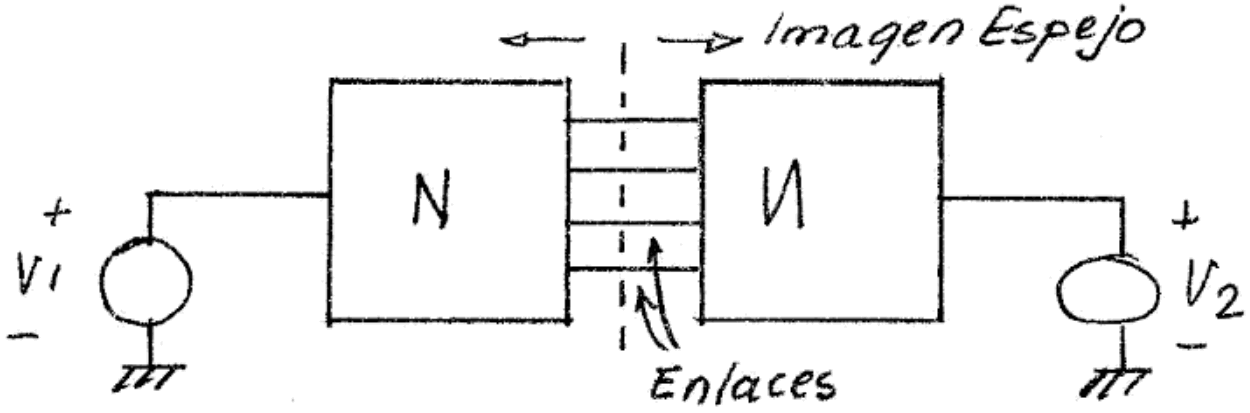
\includegraphics[width=0.8\linewidth]{_fig/multietapas_red-teorema-biseccion.png}
	\caption{Red apto para aplicar el Teorema de Bisección}
	\label{fig:multietapas_red-teorema-biseccion}
\end{figure}

El Teorema dice que cuando se aplica una señal igual o común a las dos entradas, se puede cortar los enlaces que unen las dos redes sin por eso modificar las tensiones y corrientes. En el caso de aplicar señales opuestas, la señal diferencial, se cortocircuitan los enlaces que unen los dos circuitos y se considera que se aplica una señal de valor $V_d / 2$, y de esta manera se pueden obtener las relaciones que corresponden a este caso. Esquemáticamente se representa en la Figura \ref{fig:multietapas_teorema-biseccion}.

\begin{figure}[h]
	\centering
	\subfloat[Modo Común]
	{
		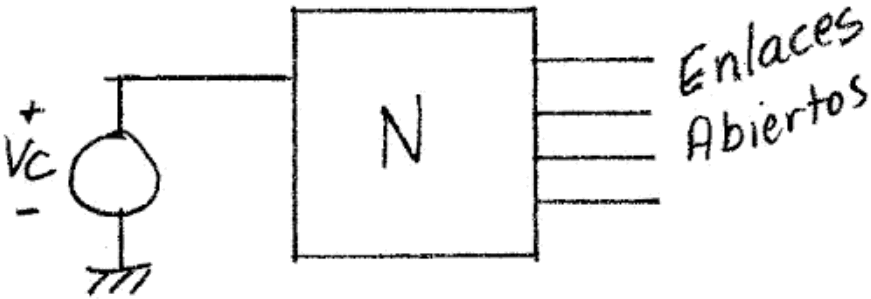
\includegraphics[width=0.46\linewidth]{_fig/multietapas_teorema-biseccion_modo-comun.png}
		\label{fig:multietapas_teorema-biseccion_modo-comun}
	}
	\subfloat[Modo Diferencial]
	{
		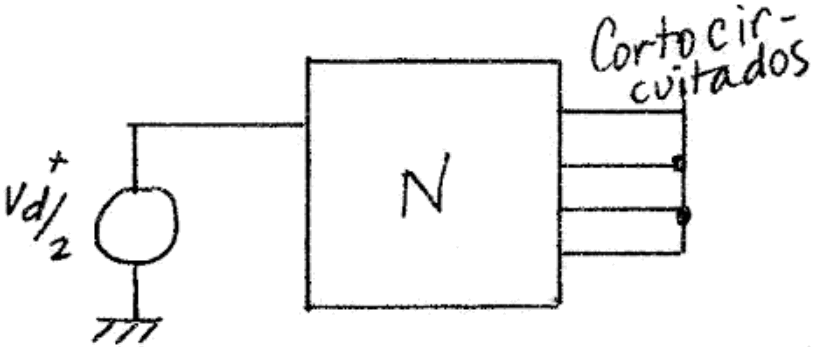
\includegraphics[width=0.46\linewidth]{_fig/multietapas_teorema-biseccion_modo-diferencial.png}
		\label{fig:multietapas_teorema-biseccion_modo-diferencial}
	}
	\caption{Aplicación de Teorema de Bisección}
	\label{fig:multietapas_teorema-biseccion}
\end{figure}

Para efectos de determinar el punto de operación y la ganancia de modo común, $A_c$, se aplica una excitación simétrica a la Figura \ref{fig:multietapas_conf-diferencial}, $V_1 = V_2 = V_c$, y resulta el equivalente de la Figura \ref{fig:multietapas_sch-teorema-biseccion_modo-comun}. De aquí se consigue:

\begin{enumerate}
	\item[a)] \( A_C = \frac{-\beta R_C}{r_{\pi} + (\beta +1)2R_E} \)
	\item[b)] \( V_E = -V_{BE} + V_{EE} \approx V_{EE} - 0.7 \)
\end{enumerate}

De donde:
\[
I_E = \frac{(V_{EE} - 0.7)}{2R_E}
\]

\begin{figure}[h]
	\centering
	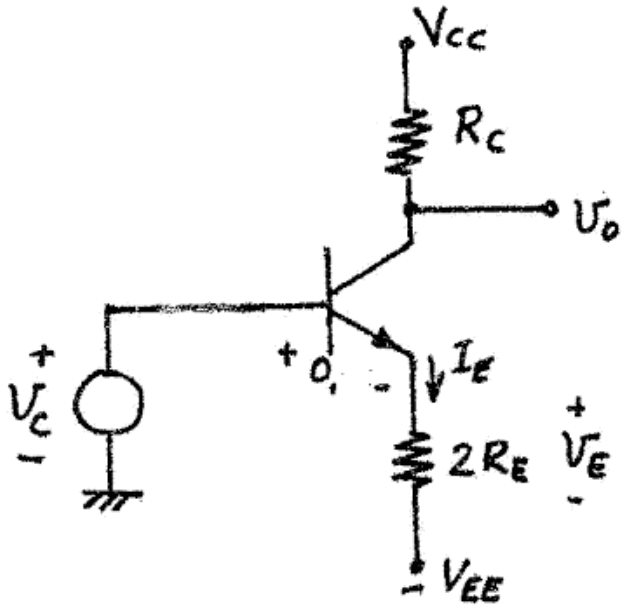
\includegraphics[width=0.6\linewidth]{_fig/multietapas_sch-teorema-biseccion_modo-comun.png}
	\caption{Teorema de Bisección, Modo común (esquema)}
	\label{fig:multietapas_sch-teorema-biseccion_modo-comun}
\end{figure}

Para hallar la ganancia y otras características de modo diferencial, se aplica una excitación antisimétrica a la Figura \ref{fig:multietapas_conf-diferencial}, \( V_1 = -V_2 = V_d/2 \), y resulta el equivalente de la Figura \ref{fig:multietapas_sch-teorema-biseccion_modo-diferencial}.

\begin{equation} \label{multietapas_ganancia-diferencial}
	A_d = \frac{-\beta R_C}{2r_{\pi}}
\end{equation}

\begin{figure}[h]
	\centering
	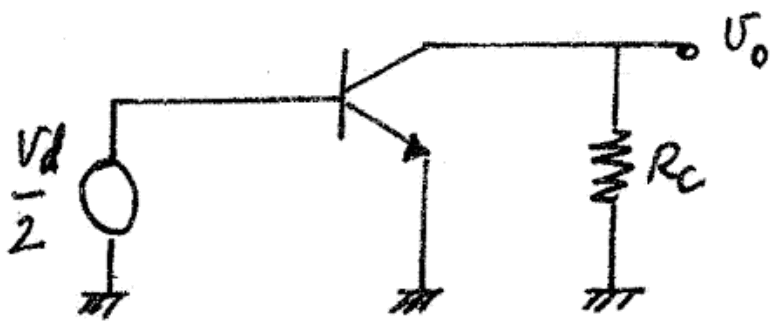
\includegraphics[width=0.8\linewidth]{_fig/multietapas_sch-teorema-biseccion_modo-diferencial.png}
	\caption{Teorema de Bisección, Modo diferencial (esquema)}
	\label{fig:multietapas_sch-teorema-biseccion_modo-diferencial}
\end{figure}

Como en el caso de la configuración EC, la resistencia \( R_E \) le proporciona estabilidad térmica al circuito, disminuyendo el cambio de \( I_C \) con cambios de temperatura; valores mayores de \( R_E \) hacen el circuito más estable. La expresión de la ganancia diferencial \ref{multietapas_ganancia-diferencial} demuestra que su valor es grande, siendo la mitad de la ganancia del EC.

El valor de la Relación de Rechazo de Modo Común para el circuito de la Figura \ref{fig:multietapas_conf-diferencial} viene dado por:

\begin{equation}
	\text{CMRR} = 20 \log \left( \frac{\beta R_L}{2(R_S + r_{\pi})} \middle/ \frac{\beta R_C}{(R_S + r_{\pi} + 2(\beta+1)R_E)} \right) 
	\approx 20 \log \left( \frac{\beta R_E}{R_S + r_{\pi}} \right)
\end{equation}

Se puede ver que la CMRR también se favorece con aumentos de \( R_E \). Sin embargo, para una \( I \) constante, cuanto más grande sea \( R_E \), más desperdicio de potencia hay debido a la caída en \( R \).

Un dispositivo que teóricamente representa una resistencia infinita, pero que tiene una caída de voltaje finita es una fuente de corriente. En la Figura \ref{fig:multietapas_fuente-corriente-transistorizada} se muestra una posible configuración. La combinación de \( R_1 \) y \( R_2 \) fija el nivel en la base del transistor. Entonces:

\[
V_3 = -V_b - V_{BE} = (-V_{EE})
\]

donde: \( V_b = R_1 V_{BE} / (R_1 + R_2) \)

Luego: \( I \equiv I_3 = \frac{V_3}{R_3} = \frac{(V_{EE} - V_b + V_{BE})}{R_3} \)

\begin{figure}[h]
	\centering
	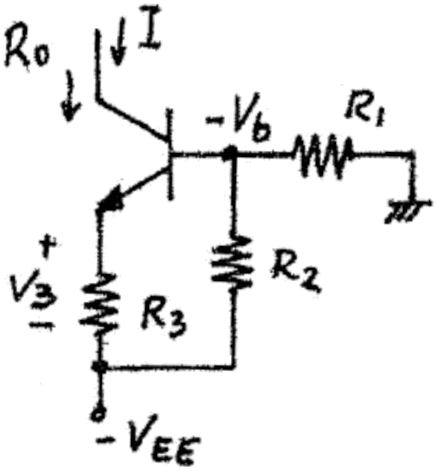
\includegraphics[width=0.4\linewidth]{_fig/multietapas_fuente-corriente-transistorizada.png}
	\caption{Fuente de Corriente Transistorizada (Reemplaza a \( R_E \) en la Figura \ref{fig:multietapas_conf-diferencial})}
	\label{fig:multietapas_fuente-corriente-transistorizada}
\end{figure}

Esta configuración se aproxima a una fuente de corriente por la impedancia alta vista desde el colector de un transistor en la región activa. La corriente que suministra es prácticamente constante y controlada por \( R_3 \). En reposo la corriente se divide en partes iguales por los transistores \( Q_1 \) y \( Q_2 \). La expresión para la resistencia de salida viene dada por (Millman-Halkias):

\begin{equation}
	R_o = \frac{(1+\beta)R_3 + R_{\phi} + r_{\pi} (1+h_{oe}R_3)}{h_{oe} (R_3 + R_{\phi} + r_{\pi} - h_{re} \beta / h_{oe})}, \quad R_{\phi} = R_1 \parallel R_2
\end{equation}

\subsubsection{Ejemplo 4}
Hallar el punto de operación, \( R_3 \) y la ganancia de modo diferencial del circuito de la Figura \ref{fig:multietapas_ejemplo4-sch}.

\begin{figure}[h]
	\centering
	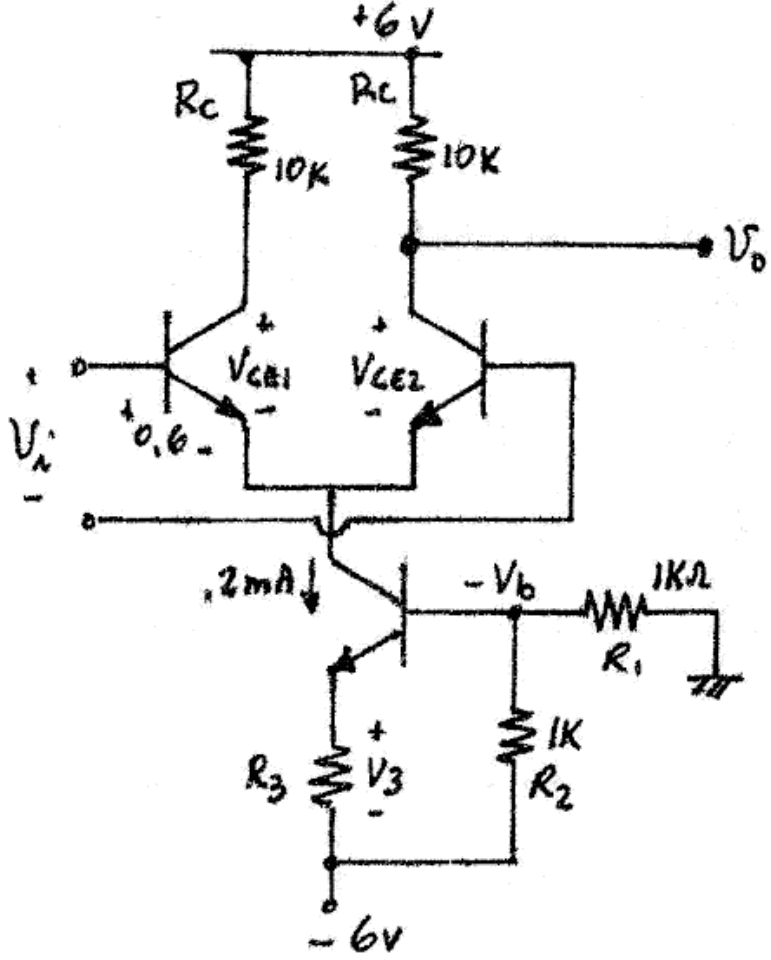
\includegraphics[width=0.7\linewidth]{_fig/multietapas_ejemplo4-sch.png}
	\caption{Circuito de Ejemplo}
	\label{fig:multietapas_ejemplo4-sch}
\end{figure}

\textbf{Solución:}

Con \( R_1 = R_2 = 1K \),

entonces: \( -V_b = \frac{-6}{2} = -3 \)

después: \( V_3 = +6 - (0.6 + 3) = +2.4V \)

y \( R_3 = \frac{V_3}{I} = \frac{2.4V}{0.2mA} = 12K\Omega \)

Entonces: \( V_{CE3} = -V_{BE1} + V_{EE} - V_3 = 3V \)

\( V_{CE1} = V_{CE2} = V_{CC} - I_C R_C - V_E = 6 - (0.1)(10K) - (-6.7) = 5.7V \)

\( g_m = \frac{I_C}{V_T} = 3.8 \times 10^{-3} \)

\( r_{\pi} = \frac{\beta}{g_m} = 26K \) (Se hace notar el valor elevado)

\( R_i = 2 r_{\pi} = 52K \)

\( A_d = \frac{+\beta R_C}{2r_{\pi}} \approx +20 \)

La junta BE de \( Q_3 \) tendrá una caída de voltaje que variará con variaciones de temperatura, que en consecuencia hará variar la corriente de la fuente. Para compensar este cambio, se puede colocar componentes en la red de polarización de base, como por ejemplo los diodos en la Figura \ref{fig:multietapas_ejemplo4_comp-termica}, con el mismo coeficiente térmico que la junta BE del transistor, de modo que no varíe la tensión en \( R_3 \), y tampoco la corriente de colector.

\begin{figure}[h]
	\centering
	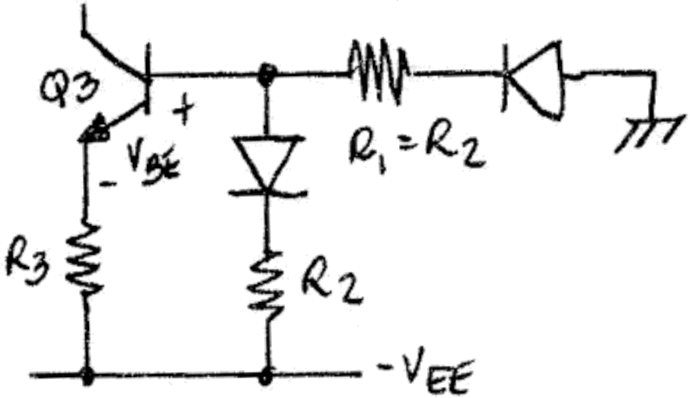
\includegraphics[width=0.6\linewidth]{_fig/multietapas_ejemplo4_comp-termica.png}
	\caption{Compensación Térmica de \( V \)}
	\label{fig:multietapas_ejemplo4_comp-termica}
\end{figure}

Encontremos ahora el \textbf{rango de modo común}. En el circuito de la Figura \ref{fig:multietapas_ejemplo4-sch}, hemos supuesto que el nivel de continua común a las entradas es 0V, y con este valor se ha obtenido \( V_{CE3} = 3V \), y \( V_{CE1} = V_{CE2} = 5.6V \). 

Si el nivel común aplicado a las entradas disminuye, se hace negativo, entonces \( V_{CE3} \) disminuye y \( V_{CE1} = V_{CE2} \) aumentan. La configuración conserva su carácter de amplificador mientras \( Q_3 \) cumple la función de una fuente de corriente, lo que exige que \( Q_3 \) permanezca en la región activa, o que:

\[
V_{CE3} > 0.2V
\]

Esto a su vez implica:

\[
V_{BI} = V_{B2} > -V_{EE} + V_3 + V_{CE3} (\text{mín}) + V_{BE}
\]

\[
V_{BI} = -6 + 3 + 0.2 + 0.7 = -2.1V
\]

Entonces, el nivel mínimo de las entradas es \( V_{BI} = V_{B2} > -2.1V \), para que \( Q_3 \) cumpla la función de fuente de corriente.

Y ¿cómo se establece el nivel máximo? A medida que aumenta \( V_{BI} = V_{B2} \), disminuye \( V_{CE1} = V_{CE2} \). Sin embargo, \( V_{CE1} \) y \( V_{CE2} \) requieren un nivel mínimo para permitir que la señal de salida pueda variar como respuesta a la señal de entrada. En el circuito de la Figura 2.27, con \( V_{BI} = V_{B2} = 0 \), entonces tenemos \( I_C = 0.1 \) mA, y \( V_{CE} = V_{CC} - I_C R_C - V_E = 6 - (0.1 \times 10) - 0.7 = 5.7V \), es decir, el punto de operación es \( (V_{CE}, I_C) = (5.7V, 0.1 \text{ mA}) \). En la Figura \ref{fig:multietapas_ejemplo4_recta-de-carga} se muestra la recta de carga. A medida que \( V_{BI} = V_{B2} \) aumenta, esta recta va desplazándose a la izquierda.

Para la mayor variación de salida se requiere que:

\[
V_{CC} - V_{EI} - I R_C > 0.2V
\]

o 

\[
V_{EI} < V_{CC} - I R_C - 0.2 = 6 - 2 - 0.2 = 3.8V
\]

Y como 

\[
V_{EI} = V_{BI} - 0.7
\]

luego 

\[
V_{BI} = V_{EI} + 0.7 > 3.8 + 0.7 = 4.5V
\]

Entonces el nivel máximo de \( V_{BI} = V_{B2} \) es 4.5V.

El Rango de Modo Común queda:

\[
-2.1V < V_{BI} = V_{B2} < 4.5V
\]

\begin{figure}[h]
	\centering
	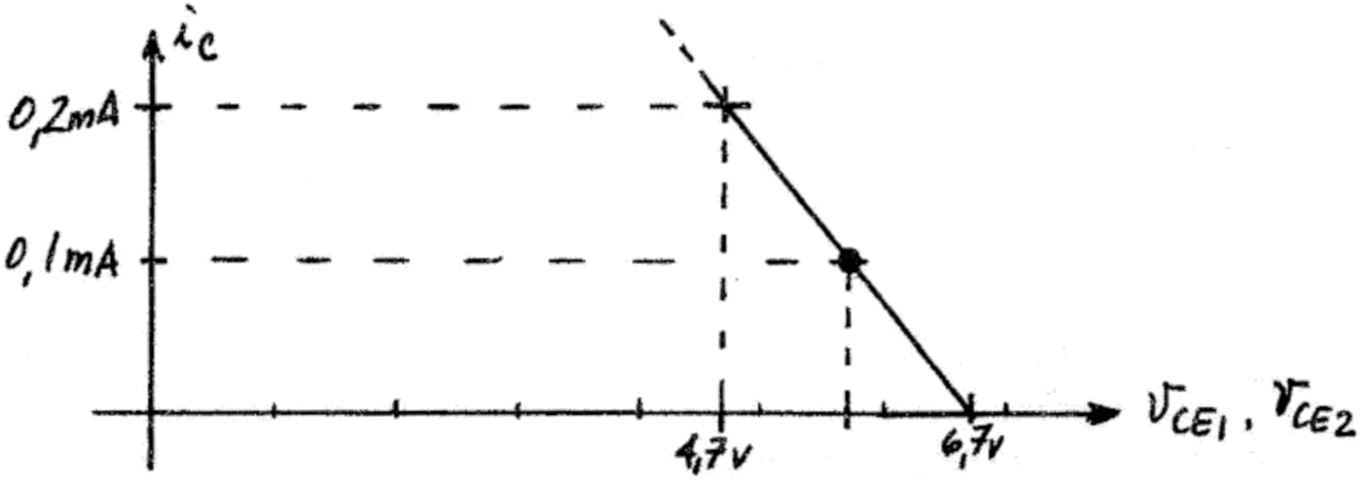
\includegraphics[width=0.8\linewidth]{_fig/multietapas_ejemplo4_recta-de-carga.png}
	\caption{Recta de Carga de \( Q_S \) en Figura \ref{fig:multietapas_ejemplo4-sch}}
	\label{fig:multietapas_ejemplo4_recta-de-carga}
\end{figure}

Otra configuración fuente de corriente, que se utiliza sobre todo en los circuitos integrados, es la denominada "espejo de corriente" que se muestra en la Figura \ref{fig:multietapas_ejemplo4_espejo-de-corriente}. Se hace notar que la base y el emisor de \( Q_1 \) y \( Q_2 \) están unidos; por lo tanto, si los transistores son idénticos, necesariamente la corriente de colector de un transistor es igual a la del otro transistor. 

\begin{figure}[h]
	\centering
	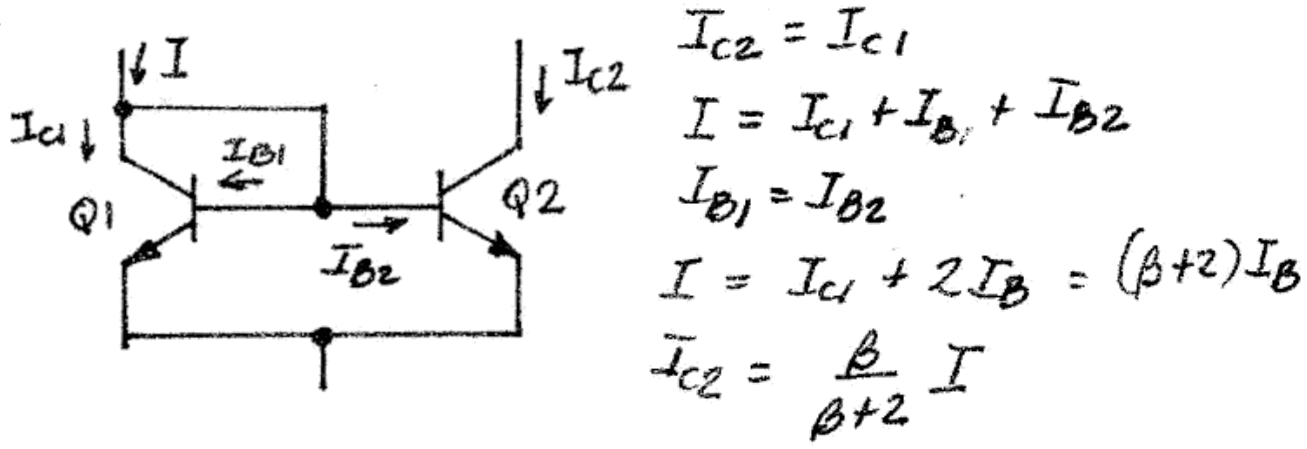
\includegraphics[width=0.8\linewidth]{_fig/multietapas_ejemplo4_espejo-de-corriente.png}
	\caption{Espejo de Corriente}
	\label{fig:multietapas_ejemplo4_espejo-de-corriente}
\end{figure}

\subsection{La característica de transferencia de la configuración diferencial} %p94

La característica de transferencia del amplificador diferencial permite determinar los límites de operación lineal para señales diferenciales. En la Figura \ref{fig:multietapas_par-diferencial-transistores}, se indican las señales de interés del conjunto, de donde se obtienen las siguientes relaciones:

\( -V_{BI} + V_{BE1} - V_{BE2} + V_{B2} = 0 \), de donde

\begin{equation}
	V_{BI} - V_{B2} = V_{BE1} - V_{BE2}
\end{equation}

e

\begin{equation}
	I_{C1} + I_{C2} = I_0 \quad \text{(una constante)}
\end{equation}

Bajo condiciones de equilibrio, \( V_{BI} = V_{B2} \), \( V_{BE1} = V_{BE2} \) e \( I_{C1} = I_{C2} = I_0 /2 \).

Cuando \( V_{BE1} < V_{\gamma} \) (voltaje umbral), \( Q_1 \) estará en la región de corte, \( I_{C1} = 0 \), y toda la corriente pasa por \( Q_2 \), \( I_{C2} = I_0 \). A medida que aumenta \( V_{BE1} \), aumenta \( I_{C1} \) y disminuye \( I_{C2} \). El rango de tensión para el cual la salida puede seguir la entrada viene dado.

\begin{figure}[h]
	\centering
	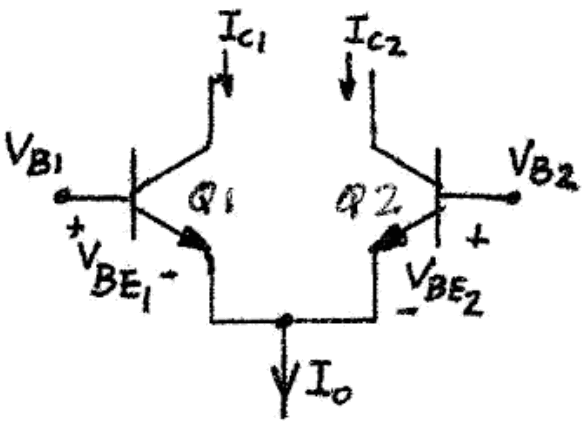
\includegraphics[width=0.5\linewidth]{_fig/multietapas_par-diferencial-transistores.png}
	\caption{La configuración diferencial}
	\label{fig:multietapas_par-diferencial-transistores}
\end{figure}

Por \( \Delta V = R_C I_{\text{TOTAL}} = R_C I_0 \)

La relación exacta entre las tensiones de entrada y las corrientes que circulan por los transistores se encuentra por medio de la ecuación de corriente de una junta \( pn \):

\begin{equation}
	I_E \approx I_S e^{V_{BE}/V_T} \tag{2.37}
\end{equation}

Se tiene

\[
I_0 = I_{E1} + I_{E2} = I_S e^{V_{BE1}/V_T} + e^{V_{BE2}/V_T} = I_S e^{(V_{BI} - V_{B2})/V_T}
\]

de donde

\begin{equation}
	I_{E2} = \frac{I_0}{(1 + e^{(V_{BI} - V_{B2})/V_T})} \tag{2.38}
\end{equation}

y por simetría,

\begin{equation}
	I_{E1} = \frac{I_0}{(1 + e^{-(V_{BI} - V_{B2})/V_T})} \tag{2.39}
\end{equation}

Estas relaciones se grafican en la Figura \ref{fig:multietapas_caracteristicas-par-diferencial}.

Se observa que:
\begin{enumerate}
	\item Cuando \( |V_{BI} - V_{B2}| > 4V_T \), \( \Delta V_T = 104 \) mV a la temperatura ambiental, el circuito ha llegado a un valor extremo, y habrá un transistor en la región de corte.
	\item La pendiente es \( I_0 / 4V_T \), la 1/4 de la de un transistor, y solo para \( |V_{BI} - V_{B2}| < 2V_T = 59 \) mV.
	\item La ganancia es proporcional a la corriente de reposo, ya que es proporcional a \( g_m R_C \); si se quiere cambiar la ganancia, esto se puede lograr modificando la corriente del punto de operación.
\end{enumerate}

\begin{figure}[h]
	\centering
	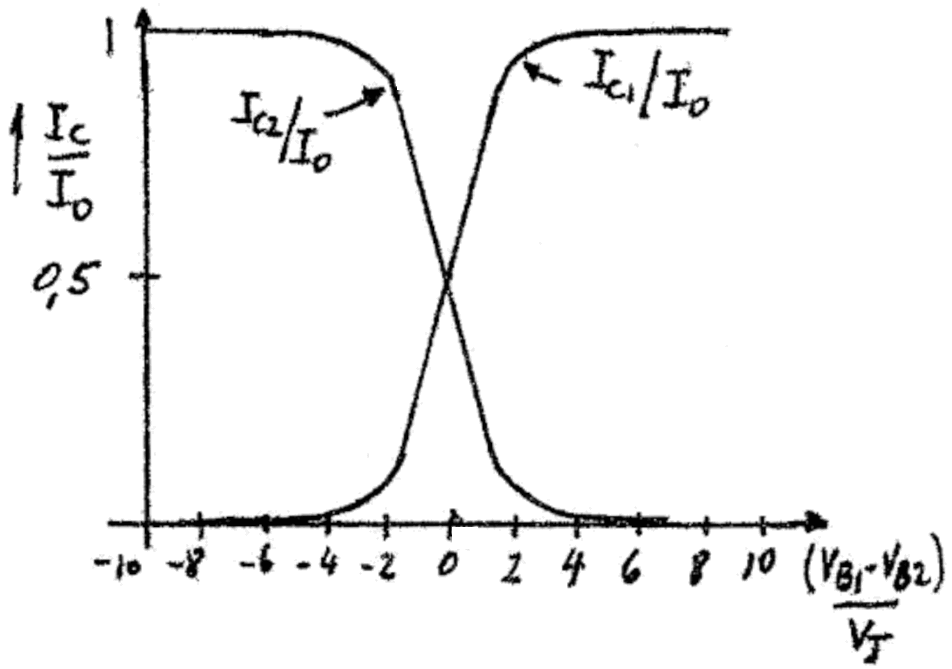
\includegraphics[width=0.8\linewidth]{_fig/multietapas_caracteristicas-par-diferencial.png}
	\caption{La configuración diferencial}
	\label{fig:multietapas_caracteristicas-par-diferencial}
\end{figure}

Hay aplicaciones donde explícitamente la entrada es sencilla pero implícitamente es diferencial, como en el siguiente ejemplo.

\subsubsection{Ejemplo 5}
Dado \( v_s(t) = 1 \sin wt \), hallar y dibujar \( v_o(t) \) del circuito de la Figura \ref{fig:multietapas_ejemplo5-sch}.

\begin{figure}[h]
	\centering
	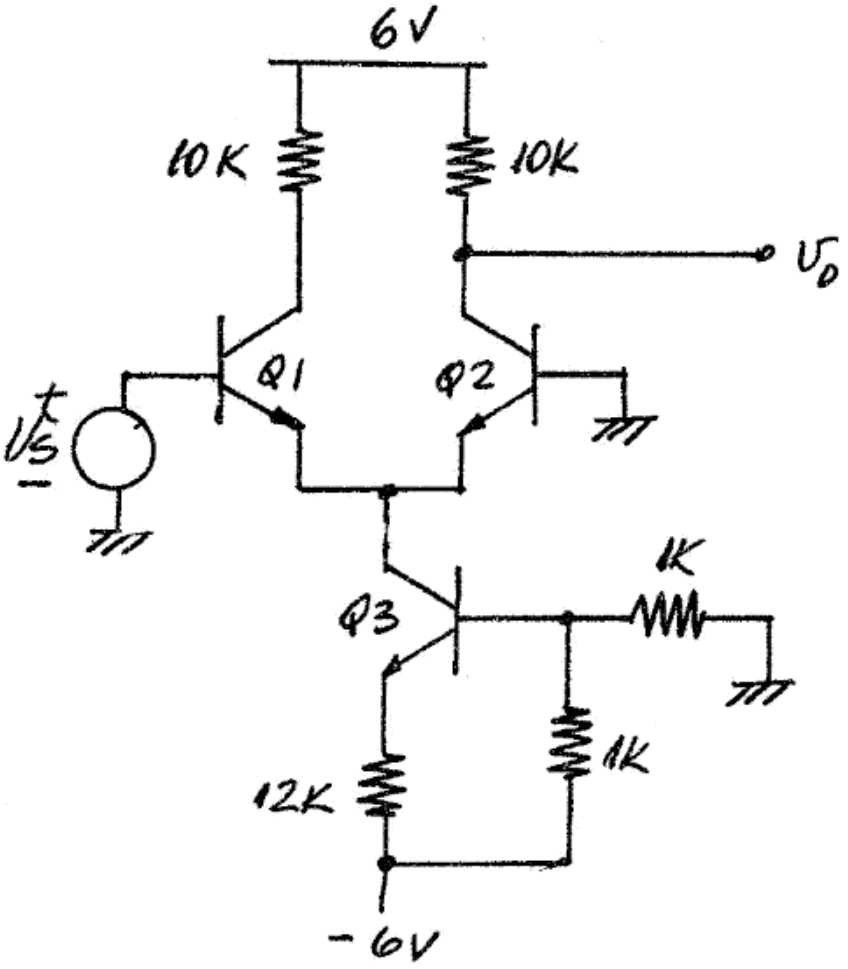
\includegraphics[width=0.4\linewidth]{_fig/multietapas_ejemplo5-sch.png}
	\caption{Circuito de Ejemplo}
	\label{fig:multietapas_ejemplo5-sch}
\end{figure}

\textbf{Solución:} A pesar de que solo aparece una entrada, podemos reconocer la configuración diferencial y analizarla como tal. Haciendo: \( V_1 = v_s \), \( V_2 = 0 \), de donde \( V_d = V_1 - V_2 = V_s \), y \( V_c = \frac{(V_1 + V_2)}{2} = \frac{V_s}{2} \).

Entonces el circuito es el mismo de la Figura \ref{fig:multietapas_ejemplo4_comp-termica}; la fuente de corriente suministra \( 0.2 \text{mA} \), que en condiciones de reposo se reparte equitativamente entre los 2 transistores, de modo que \( V_o (\text{DC}) = 6V - 10K(0.1mA) = 5V \). La fuente de corriente \( Q_3 \) hace que la ganancia de modo común sea prácticamente igual a 0. Entonces, si \( A_c \approx 0 \) y \( v_d = v_s \), nos queda \( v_o = A_d v_s \), donde \( A_d \) necesariamente es positiva.

Si se aplica el Teorema de Bisección, nos queda el siguiente circuito, la Figura \ref{fig:multietapas_ejemplo5-biseccion}.

\begin{figure}[h]
	\centering
	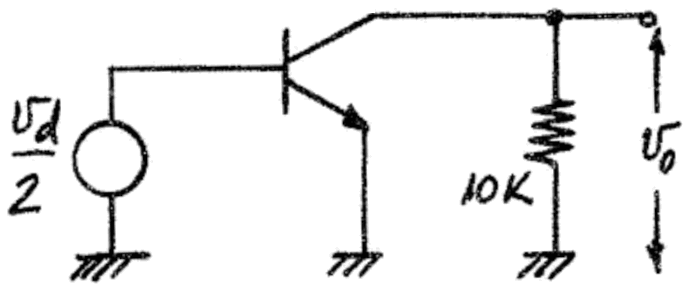
\includegraphics[width=0.6\linewidth]{_fig/multietapas_ejemplo5-biseccion.png}
	\caption{Aplicando Teorema de Bisección}
	\label{fig:multietapas_ejemplo5-biseccion}
\end{figure}

De aquí:

\[
\frac{v_o}{(v_d /2)} = -\beta \cdot 10K / V_T = - g_m 10k = - 0.1mA \cdot 10K / 25mV
\]

o 

\[
A_d = \frac{v_o}{v_d} = -1K / 50 = -20.
\]

En la zona lineal, la ganancia \( v_o / v_s = 20 \). La zona lineal es de una extensión limitada, ya que de su valor de \( 5V \) en DC, \( v_o \) solo puede variar hasta \( 6V \) en una dirección (\( i_{C2} = 0 \)), y hasta \( 4V \) en la otra (\( i_{C2} = 0.2mA, i_{C1} = 0 \)). Es decir, la máxima variación de \( v_o \) es \( 1V \) en cada dirección.

Para causar esta variación, \( v_s \) variará \( 1V / 20 = 50mV \). Mientras \( v_s > 50mV \), entonces \( v_o = 6V \), y cuando \( v_s < -50mV \), \( v_o = 4V \). Habrá solo un trayecto corto de \( v_s \) en que se amplifica linealmente. El resultado se muestra en la Figura \ref{fig:multietapas_ejemplo5-respuesta}.

\begin{figure}[h]
	\centering
	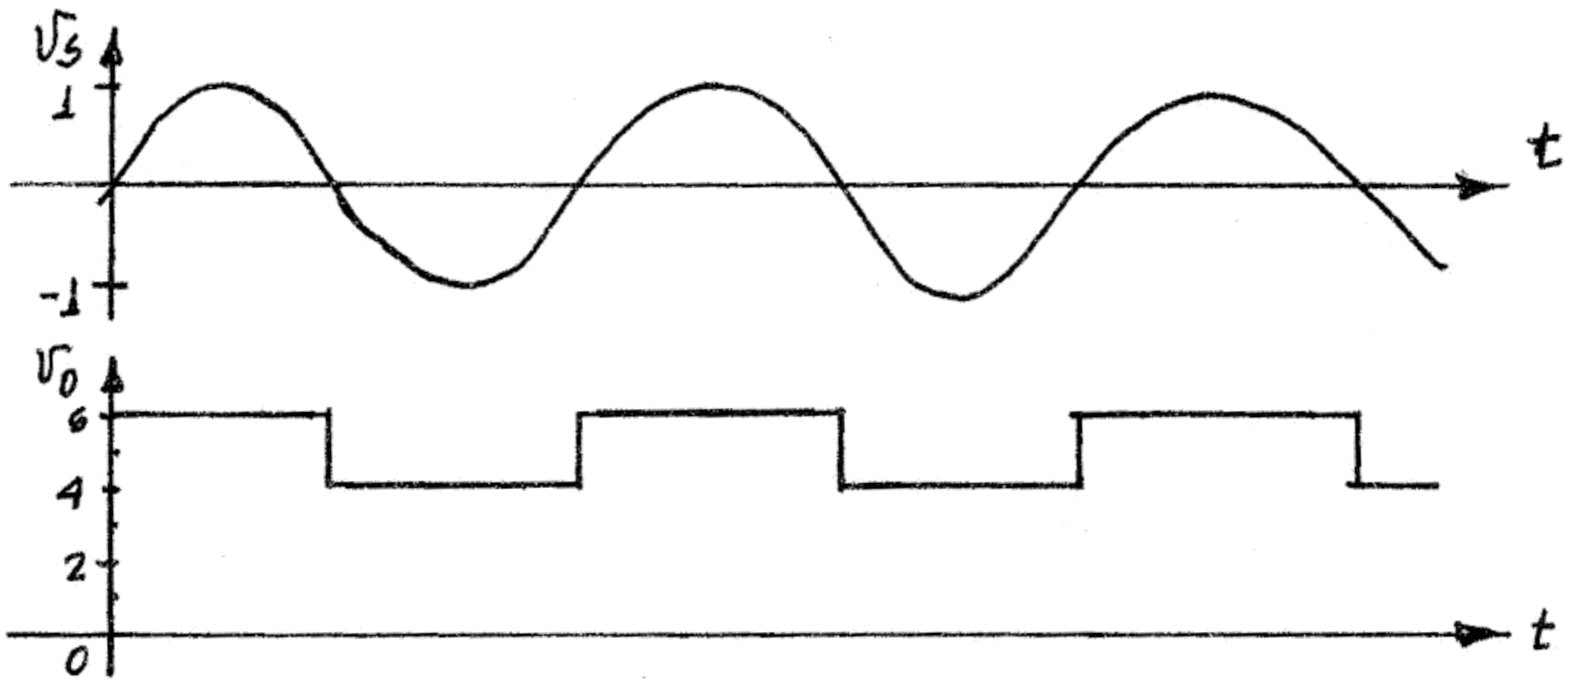
\includegraphics[width=0.8\linewidth]{_fig/multietapas_ejemplo5-respuesta.png}
	\caption{Respuesta \( V_s \) y \( V_o \)}
	\label{fig:multietapas_ejemplo5-respuesta}
\end{figure}

En resumen, la configuración diferencial anterior es una solución excelente a los requerimientos de un amplificador de corriente contínua, con buena ganancia y buena estabilidad térmica. Esta configuración simétrica con salida sencilla a su vez ha dado lugar a modificaciones por diversos motivos. A continuación la analizaremos cuando la salida es diferencial y cuando el circuito no es simétrico.

\subsection{Configuración entrada diferencial, salida diferencial} %p98

En la Figura \ref{fig:multietapas_amp-diferencial_salida-diferencial} se representa un esquema de este tipo de circuito

\begin{figure}[h]
	\centering
	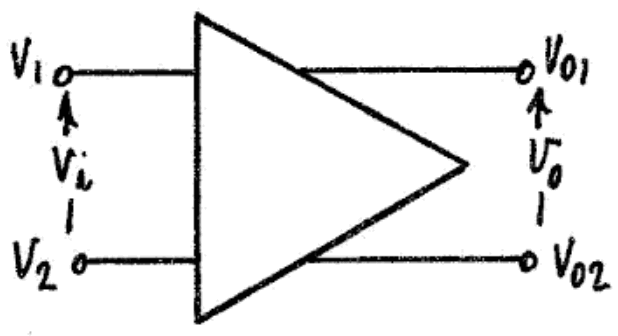
\includegraphics[width=0.4\linewidth]{_fig/multietapas_amp-diferencial_salida-diferencial.png}
	\caption{Amplificador Diferencial con Salida Diferencial}
	\label{fig:multietapas_amp-diferencial_salida-diferencial}
\end{figure}

Tenemos:

\[ 
V_o = V_{o1} - V_{o2}
\]

\[ 
V_{o1} = A_{11} V_1 + A_{21} V_2
\]

\[
V_{o2} = A_{12} V_1 + A_{22} V_2
\]

de donde

\[
V_o = (A_{11} - A_{12}) V_1 + (A_{21} - A_{22}) V_2
\]

Para circuitos simétricos se cumple que:

\begin{equation} \label{equ:multietapas_amp-diferencial_salida-diferencial_relacion}
	A_{22} = A_{11} \quad \text{y} \quad A_{21} = A_{12}
\end{equation}

de donde \( A_{11} - A_{12}) = -(A_{21} - A_{22}) \)
y \( V_o = (A_{11} - A_{22})(V_1 - V_2) = A_d V_d \)

es decir, la ganancia de modo común es idénticamente igual a \( 0 \).

La salida diferencial elimina cualquier componente común.

Si hay diferencias de los componentes, entonces las relaciones de la ecuación \ref{equ:multietapas_amp-diferencial_salida-diferencial_relacion} no son correctas. Por ejemplo, si:

\begin{equation}
	A_{22} = A_{11} + \Delta_1 \quad \text{y} \quad A_{21} = A_{12} + \Delta_2
\end{equation}

entonces,

\[
V_o = (A_{11} - A_{12})V_1 - (A_{11} - A_{12})V_2 + (\Delta_2 - \Delta_1)
\]	
\[
V_o = (A_{11} - A_{12})(V_1 - V_2) + (\Delta_2 - \Delta_1)V_2
\]

de donde evidentemente habrá una ganancia de modo común.

\subsection{Circuito diferencial no simétrico} %p99

Existen configuraciones diferenciales que no son perfectamente simétricas como en los circuitos anteriores. Para tales circuitos el Teorema de Bisección no es aplicable sencillamente por que no se cumplen las condiciones necesarias para su aplicación. Tendremos la obligación de analizar el circuito de otra forma. A continuación veremos varios casos utilizando 1) Circuito diferencial con la salida no balanceada, 2) Circuito diferencial con la fuente no balanceada.

\subsection{Circuito diferencial no Balanceado - Uso de Modelo de Pequeña Señal} %p99

En la Figura \ref{fig:multietapas_conf-diferencial_modelo} tenemos un configuración diferencial, en donde los circuitos de base son simétricos, y la polarización de los emisores con fuentes de corriente es simétrica. Sin embargo, los circuitos de colector son distintos. Se puede analizar este circuito si se resuelve como un todo, reemplazando los transistores por su modelo equivalente y trabajando con el conjunto resultante de nodos y mallas. Para este circuito, nos queda el equivalente de la Figura \ref{fig:multietapas_conf-diferencial_equivalente}.

\begin{figure}[h]
	\centering
	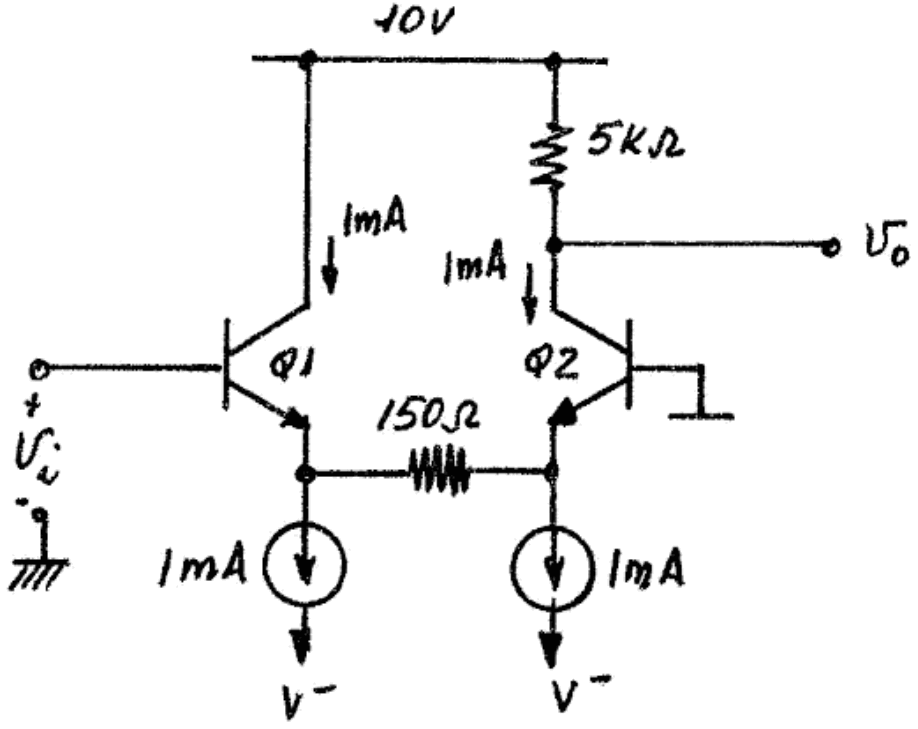
\includegraphics[width=0.6\linewidth]{_fig/multietapas_conf-diferencial_modelo.png}
	\caption{Configuración diferencial, circuito}
	\label{fig:multietapas_conf-diferencial_modelo}
\end{figure}

\begin{figure}[h]
	\centering
	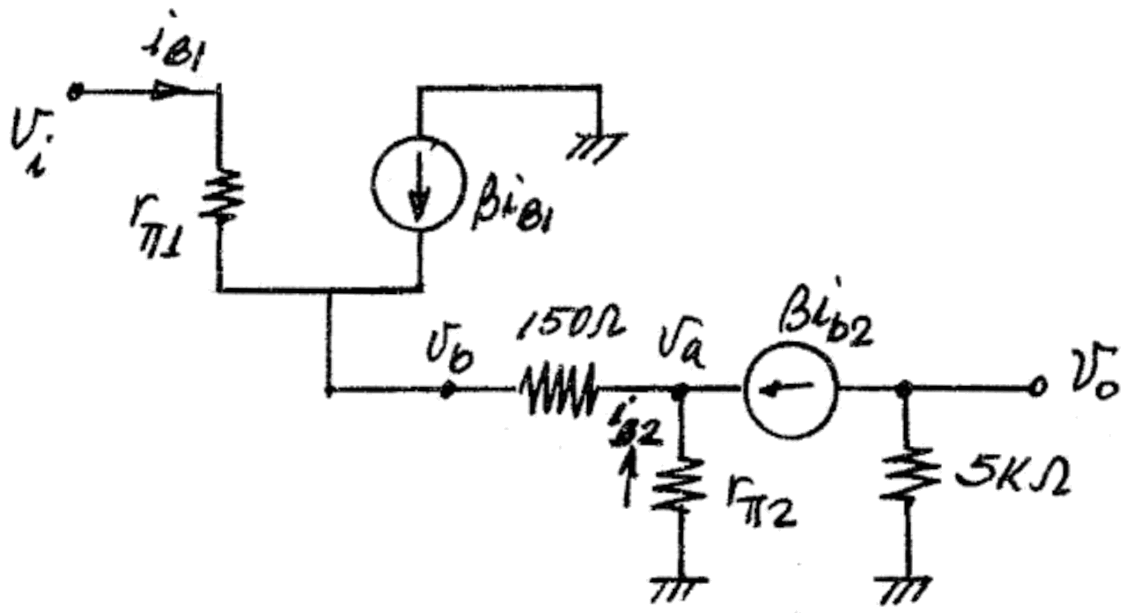
\includegraphics[width=0.6\linewidth]{_fig/multietapas_conf-diferencial_equivalente.png}
	\caption{Configuración diferencial, equivalente}
	\label{fig:multietapas_conf-diferencial_equivalente}
\end{figure}

De ésta figura se obtiene
\[
V_o/V_a = 85k/r_{\pi 2}
\]
\[
V_a/V_b = (r_{\pi 2}/(\beta+1))/(150 + r_{\pi 2}/(\beta+1))
\]
\[
V_b/V_i = (\beta+1)(150 + r_{\pi 2}/(\beta+1)) / (r_{\pi 1} + (\beta+1)(150 + r_{\pi 2}/(\beta+1)))
\]
\[
V_o/V_i = 85K/(r_{\pi 1} + (\beta+1)(150 + r_{\pi 2}/(\beta+1)))
\]

con \( r_{\pi 2} = 100 \cdot 25 \text{mV}/1 \text{mA} = 2500 \Omega \)

da \( V_o/V_i = 25 \)

y \( R_i = r_{\pi 1} + (\beta+1)(150 + r_{\pi 2}/(\beta+1)) = 20.2K\Omega \)

\subsubsection{Ejercicio 6}

Compare el circuito de la Figura \ref{fig:multietapas_ejemplo6-sch-a} con el de la Figura \ref{fig:multietapas_ejemplo6-sch-b}. Sin necesidad de hacer cálculos, ¿cuál de los dos circuitos presenta mayor ancho de banda? ¿Por qué?, ¿El circuito con peor ancho de banda tendrá alguna característica mejor para compensar su defecto?

\begin{figure}[h]
	\centering
	\subfloat[A]
	{
		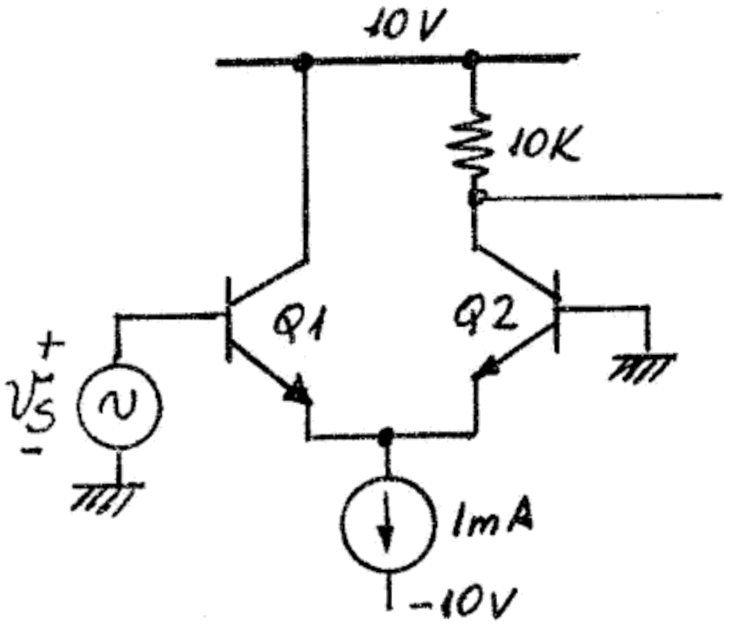
\includegraphics[width=0.46\linewidth]{_fig/multietapas_ejemplo5-sch-a.png}
		\label{fig:multietapas_ejemplo6-sch-a}
	}
	\subfloat[B]
	{
		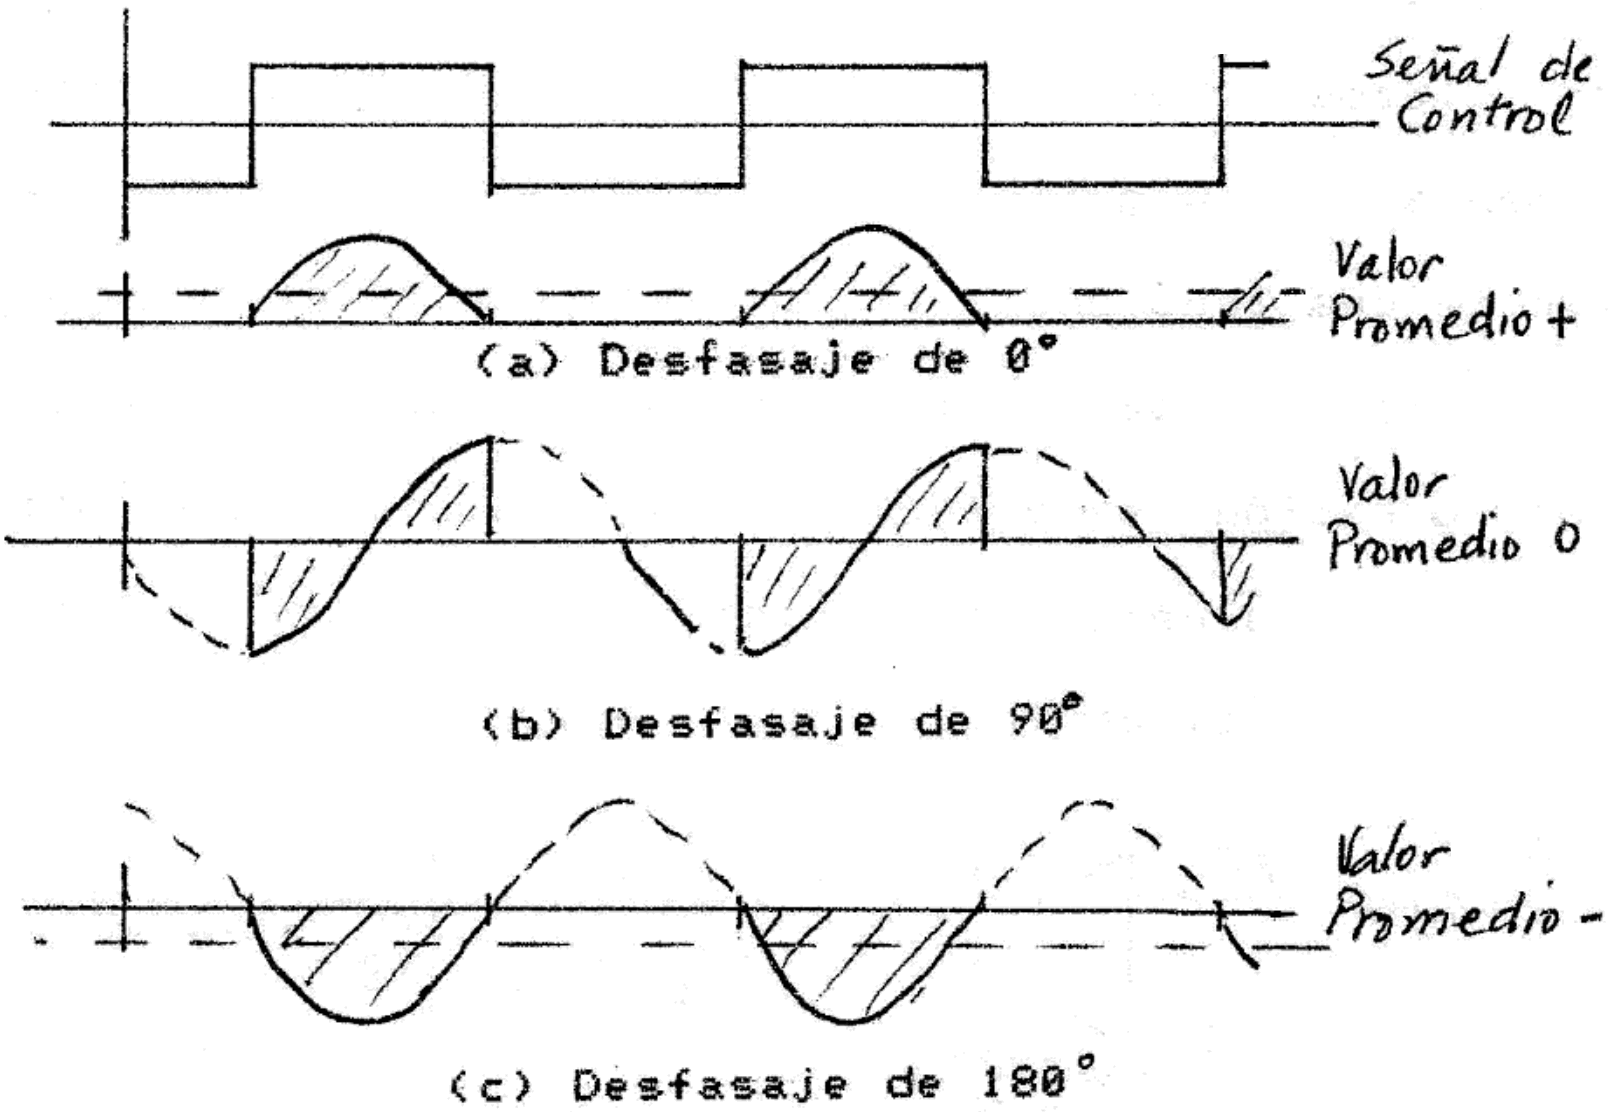
\includegraphics[width=0.46\linewidth]{_fig/multietapas_ejemplo5-sch-b.png}
		\label{fig:multietapas_ejemplo6-sch-b}
	}
	\caption{Circuito de ejemplo}
	\label{fig:multietapas_ejemplo6-sch}
\end{figure}


\subsection{Circuito diferencial no Balanceados las Fuentes de Entrada} %p101

En la Figura \ref{fig:multietapas_conf-diferencial_no-bal} se observa que el circuito de base de Q1 tiene una resistencia de 10k que no aparece en la base de Q2. Por lo tanto están desbalanceados los circuitos de polarización y

\begin{figure}[h]
	\centering
	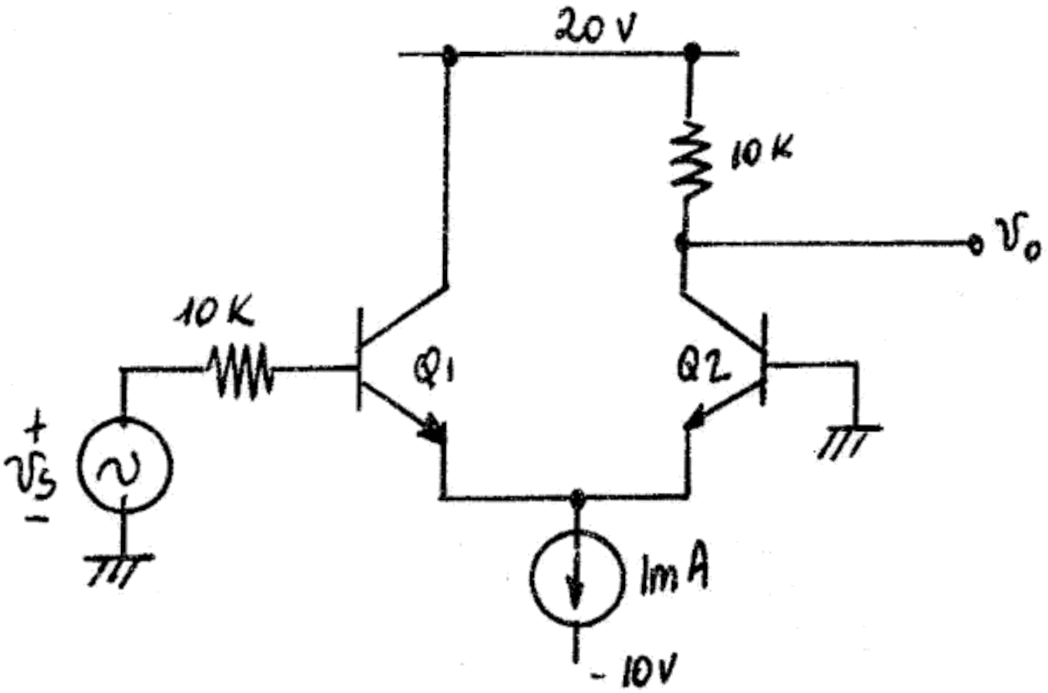
\includegraphics[width=0.4\linewidth]{_fig/multietapas_conf-diferencial_no-bal.png}
	\caption{Configuración diferencial, equivalente}
	\label{fig:multietapas_conf-diferencial_no-bal}
\end{figure}

la corriente de polarización de la fuente de corriente no va circular en partes iguales por ambos transistores. Para hallar el punto de operación, tenemos la ecuación de malla

\begin{equation} \label{equ:conf-diferencial_no-bal_malla}
	(i_{E1}/(\beta+1))10k + v_{BE1} = v_{BE2}
\end{equation}

y la ecuación de nodo

\begin{equation} \label{equ:conf-diferencial_no-bal_nodo}
	i_{E1} + i_{E2} = 1 \text{mA}
\end{equation}

con la salvedad que en lugar de tomar $v_{BE}$ fijo, es necesario considerar la pequeña diferencia que surge al circular diferentes cantidades de corriente de acuerdo a la relación

\[
v_{BE} = v_T \ln(i_E/I_S)
\]

En este caso no hace falta conocer $I_S$ ya que se requiere solamente la diferencia entre $v_{BE1}$ y $v_{BE2}$ de donde desaparece el parámetro $I_S$, como en la siguiente ecuación

\[
v_{BE1} - v_{BE2} = v_T \ln(i_{E1}/i_{E2})
\]

y la ecuación \ref{equ:conf-diferencial_no-bal_malla} se convierte en

\[
(i_{E1}/(\beta+1))10k + v_T \ln(i_{E1}/i_{E2}) = 0
\]

e incorporando la ecuación \ref{equ:conf-diferencial_no-bal_nodo} queda

\[
(i_{E1}/(\beta+1))10k + v_T \ln(i_{E1}/(1\text{mA} - i_{E1})) = 0
\]

Esta es una ecuación no-lineal, cuya solución se encuentra iterativamente, tal como se indica en la siguiente tabla:

\begin{center}
	\begin{tabular}{ccc}
		\hline
		1 & 2 & 3 \\
		\hline
		$i_{E1}$ & $(i_{E1}/(\beta+1))10k$ & $V_T \ln(i_{E1}/(1\text{mA} - i_{E1}))$ \\
		\hline
		0.49 & 0.0485 & -0.00104 \\
		0.45 & 0.0445 & -0.0052 \\
		0.4 & 0.0396 & -0.0105 \\
		0.35 & 0.0346 & -0.016 \\
		0.3 & 0.0297 & -0.022 \\
		0.26 & 0.02574 & -0.0271 \\
		0.27 & 0.02673 & -0.02586 \\
		\hline
	\end{tabular}
\end{center}

En esta tabla se procura hacer el valor de la columna 2 igual al valor negativo de la columna 3. Con el valor inicial de $i_{E1}$ el valor absoluto de la columna 2 es muy superior al valor absoluto de la columna 3. A medida que disminuye $i_{E1}$, disminuye el valor absoluto de la columna 2 y aumenta el valor absoluto de el valor absoluto de la columna 2 y aumenta el valor absoluto de la columna 3. En la penúltima fila, la columna 3 supera en valor a la columna 2; de aquí en adelante se va ajustando el valor de $i_{E1}$ en la dirección apropiada hasta lograr una cierta precisión en la diferencia entre la columna 2 y 3. Se hace notar la relación entre $i_{E1}$ e $i_{E2}$ que en vez de estar equilibradas las corrientes, tenemos \( i_{E1} = 0.27 \text{mA} \) e \( i_{E2} = 0.73 \text{mA}\).

\subsubsection{Ejemplo 7}
Para el circuito de la Figura \ref{fig:multietapas_ejemplo7-sch}:

\begin{enumerate}
	\item[a)] Hallar \( I \)
	\item[b)] Hallar la corriente de polarización de entrada
	\item[c)] Hallar el Rango de Modo Común de Entrada
	\item[d)] Hallar la Resistencia de Entrada Diferencial
	\item[e)] Hallar la Ganancia Diferencial
	\item[f)] Hallar la Ganancia de Modo Común si las \( RC \) son parejas en un \( 1\% \) y si \( R_o \) de \( Q3 \) es \( 5.9 M\Omega \)
	\item[g)] Hallar la Relación de Rechazo de Modo Común
\end{enumerate}

\begin{figure}[h]
	\centering
	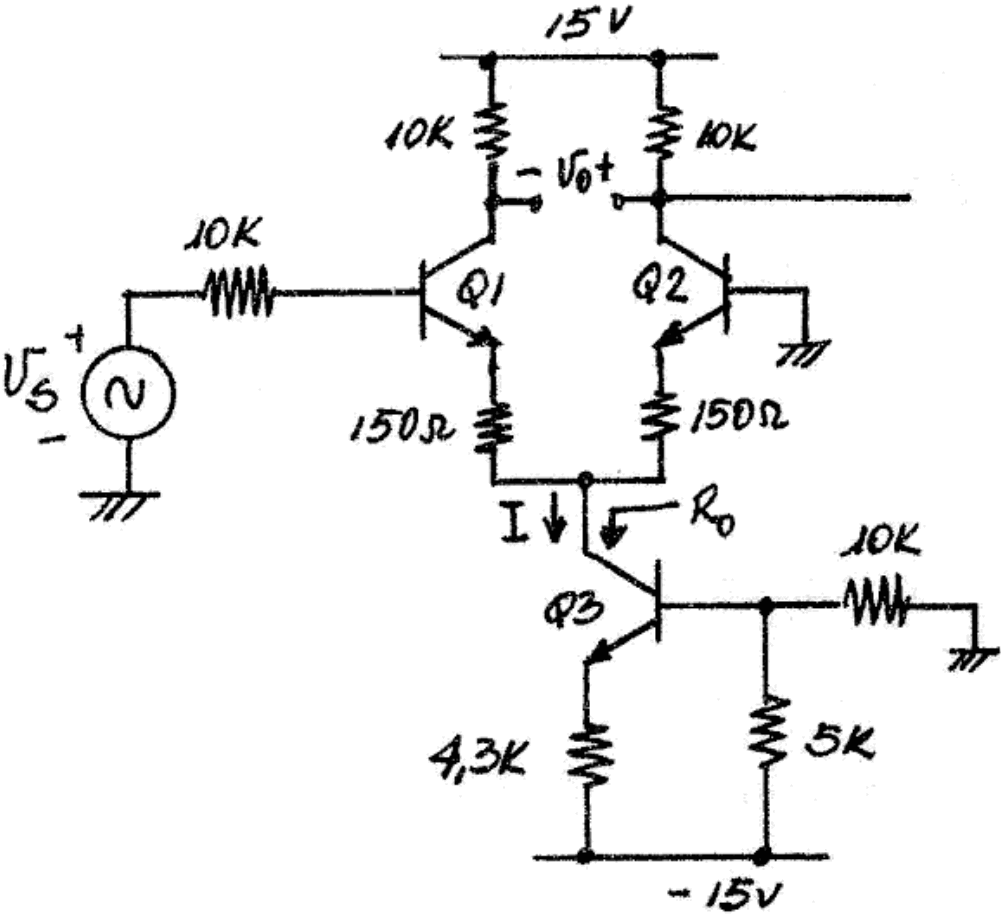
\includegraphics[width=0.6\linewidth]{_fig/multietapas_ejemplo7-sch.png}
	\caption{Circuito de Ejemplo}
	\label{fig:multietapas_ejemplo7-sch}
\end{figure}

\textbf{Solución:}

\textbf{a)} Para hallar I se crea un circuito equivalente de Thevenin en la base de Q3, quedando $R_{Th} = 10k // 5k = 3,33k$, $V_{Th} = -10V$, de donde $I_{E3} = (15 - 10 - 0,7)/(4,3k + 3,3k/101) \approx 1$ mA

\textbf{b)} Si I se divide en partes iguales, implica cada transistor se polariza con 0,5 mA de donde $i_B = 5 \mu A$. Sin embargo en este caso se observa que los circuitos de base no son simétricos por lo que requiere precisar iterativamente la distribución de I. Tenemos el siguiente par de ecuaciones:

\[
(i_{E1}/101)10k + v_{BE1} + i_{E1}150 = v_{BE2} + i_{E2}150
\]
\[
i_{E1} + i_{E2} = 1 \text{mA}
\]

y su resolución da \( i_{E1} = 0.4 \text{mA}\) e \( i_{E2} = 0.6 \text{mA} \), con lo que \( v_{BE1} = 0.695 V \) y \( v_{BE2} = 0,705 V \).

\textbf{c)} El límite inferior del rango de modo común lo determina la región activa de \( Q3 \). Si se toma saturación como \( v_{CE} = 0.2 V \), entonces \( Q3 \) entra en saturación cuando \( V_{B3} = -10.7 + 0.2 = -10.5 V \) que conlleva a \( V_{B1} = V_{B2} = -10.5 + 0.7 = -9.8 V \).

El límite superior se establece con mantener \( Q1 \) y \( Q2 \) en la región activa aún bajo la condición de la máxima excursión de la señal de salida, \( \Delta V = \Delta i_C R_C = 1 \text{mA}(10k) = 10 V \). Entonces la tensión mínima en el colector de uno de estos transistores es \( 15 - 10 = 5V \), y el nivel común de entrada máximo será \( 5 - 0.2 + 0.7 = 5.5 V \).

El rango de modo común es \( -9.3V, 5.5V) \).

\textbf{d)} La resistencia de entrada diferencial se destaca del siguiente diagrama, de donde , ver Figura \ref{fig:multietapas_ejemplo7-sch-rid}.

\begin{figure}[h]
	\centering
	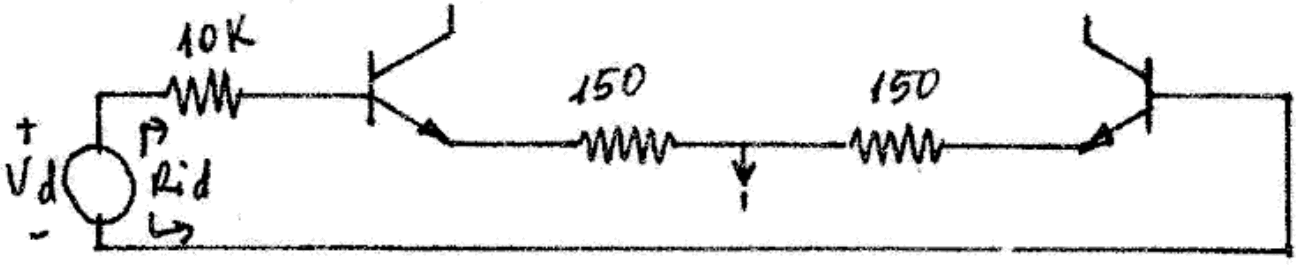
\includegraphics[width=0.6\linewidth]{_fig/multietapas_ejemplo7-sch-rid.png}
	\caption{Circuito de Ejemplo}
	\label{fig:multietapas_ejemplo7-sch-rid}
\end{figure}

\textbf{e)} La ganancia de modo diferencial la encontraremos de dos modos: por medio del modelo de pequeña señal, y utilizando el Teorema de Bisección.

En la Figura \ref{fig:multietapas_ejemplo7-pequena-senal}, se plantea el modelo de pequeña señal del circuito anterior. De aquí se obtiene:

\[
\frac{V_o^+}{V_s} = (\frac{V_o^+}{V_a})(\frac{V_a}{V_b})(\frac{V_b}{V_s})
\]
\[
\frac{V_o^+}{V_s} = 192.3 \times 0.1465 \times 0.7 = 19.7
\]

\[
\frac{V_o^-}{V_s} = \frac{-810k}{(10k + r_{\pi 1} + (\beta+1)(300 + r_{\pi 2}/(\beta+1)))} = -19.72
\]
\[
\frac{V_o}{V_s} = \frac{V_o^+ - V_o^-}{V_s} = 19.72 - (-19.72) = 39.94
\]

\begin{figure}[h]
	\centering
	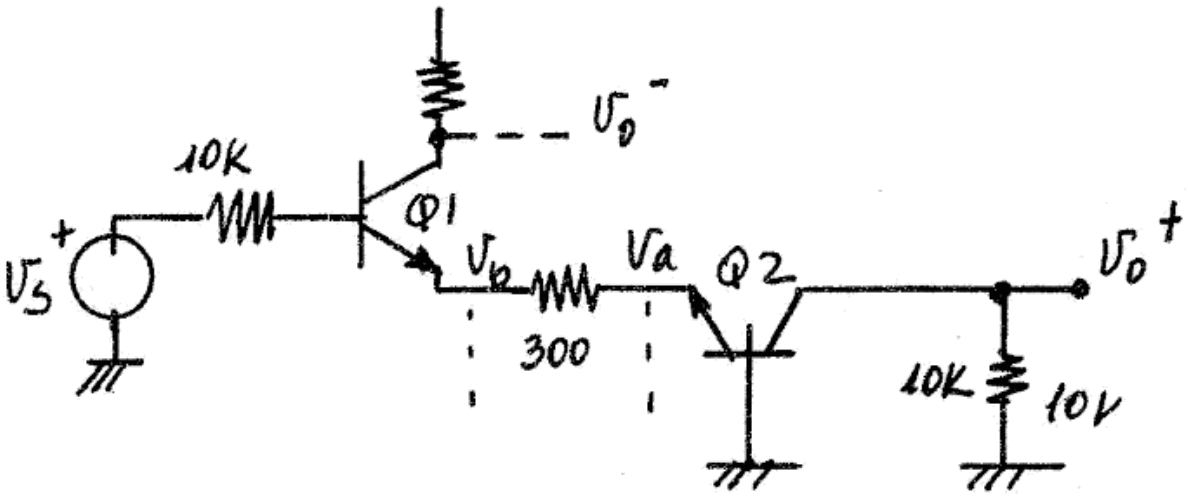
\includegraphics[width=0.4\linewidth]{_fig/multietapas_ejemplo7-pequena-senal.png}
	\caption{Circuito de Ejemplo, aplicando modelo de pequeña señal}
	\label{fig:multietapas_ejemplo7-pequena-senal}
\end{figure}

Con el Teorema de Bisección, trabajamos con el circuito como si no existiera la resistencia de \( 10K\Omega \), tal como se indica en la Figura \ref{fig:multietapas_ejemplo7-biseccion-a}, con el cual se obtiene \( V_o/V_d = 49.5 \). Posteriormente se aplica la fuente con su resistencia de \( 10K\Omega \) en serie, para quedarnos con una cascada de redes, como en la Figura \ref{fig:multietapas_ejemplo7-biseccion-b}, cuya ganancia global es

\begin{figure}[h]
	\centering
	\subfloat[A]
	{
		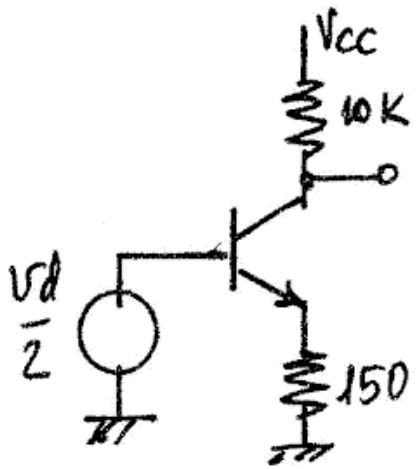
\includegraphics[width=0.46\linewidth]{_fig/multietapas_ejemplo7-biseccion-a.png}
		\label{fig:multietapas_ejemplo7-biseccion-a}
	}
	\subfloat[B]
	{
		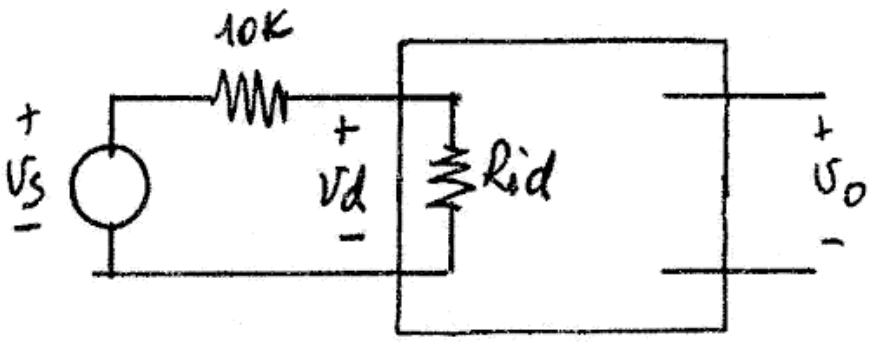
\includegraphics[width=0.46\linewidth]{_fig/multietapas_ejemplo7-biseccion-b.png}
		\label{fig:multietapas_ejemplo7-biseccion-b}
	}
	\caption{Circuito de ejemplo}
	\label{fig:multietapas_ejemplo7-biseccion}
\end{figure}

\[
v_o/v_s = (v_o/v_d)(v_d/v_s) = 49,5(40,4k)/(50,4k) = 39,76
\]

es decir, prácticamente el mismo resultado anterior.

\textbf{f)} En teoría esta configuración no tiene una ganancia de modo común excepto por diferencias en el emparejamiento de los componentes. Con $R_e$ disparejos, y considerando a $R_o$ de Q3 = 5,9 M$\Omega$, la ganancia de modo común viene dada por

\[
A_{cm} = (R_e/2R_o)(\Delta R_C/R_C) 
\]
\[
A_{cm} = 10k(0,01)/2 \times 5,9 \times 10^6 = 8,47 \times 10^{-6}
\]

\textbf{g)} La Relación de Rechazo de Modo Común viene dada por:

\[
\text{CMRR} = 20 \log |39,44/8,47 \times 10^{-6}| = 133 \text{ dB}
\]

\subsection{Par Diferencia con FET} %p106

En la Figura \ref{fig:multietapas_conf-diff-fet} se muestra una configuración diferencial con FET.

\begin{figure}[h]
	\centering
	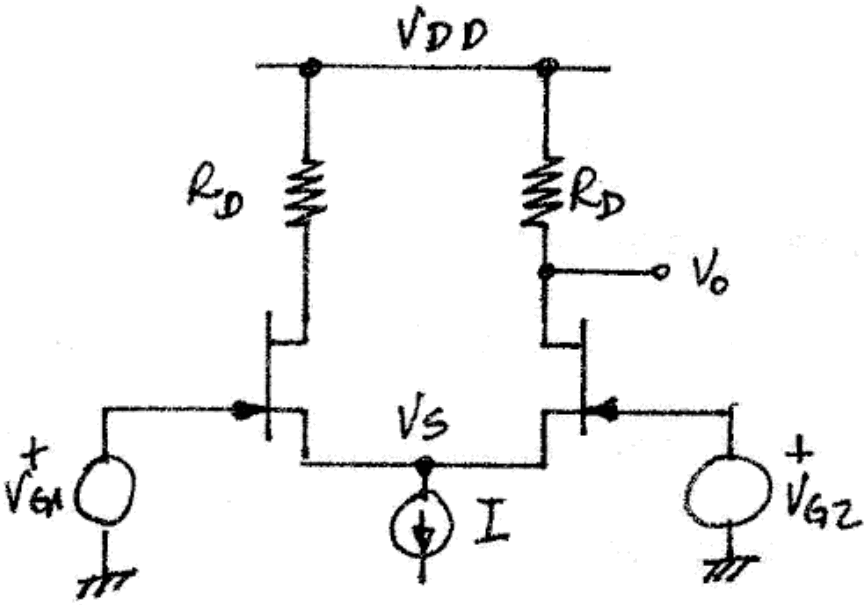
\includegraphics[width=0.4\linewidth]{_fig/multietapas_conf-diff-fet.png}
	\caption{Circuito configuracion diferencial con FET}
	\label{fig:multietapas_conf-diff-fet}
\end{figure}

Si se supone los transistores en la región de saturación entonces:

\begin{equation}
	i_{D1} = i_{DSS}(1 - \frac{v_{GS1}}{V_p})^2 = i_{DSS}(1 - \frac{v_{G1} - v_s}{V_p})^2
\end{equation}
\begin{equation}
	i_{D2} = i_{DSS}(1 - \frac{v_{GS2}}{V_p})^2 = i_{DSS}(1 - \frac{v_{G2} - v_s}{V_p})^2
\end{equation}
\begin{equation}
	\sqrt{i_{D1}} = \sqrt{i_{DSS}}(1 - \frac{v_{GS1}}{V_p})
\end{equation}
\begin{equation}
	\sqrt{i_{D1}} - \sqrt{i_{D2}} = \sqrt{i_{DSS}}(\frac{v_{GS2} - v_{GS1}}{-V_p}) = \sqrt{i_{DSS}}(\frac{v_{id}}{-V_p})
\end{equation}

pero $i_{D1} + i_{D2} = I$. Entonces de la ecuación anterior

\begin{equation}
	i_{D1} = \frac{I}{2} + v_{id} \sqrt{\frac{2I_{DSS}}{I}} - (\frac{v_{id}}{V_p})^2 (\frac{I_{DSS}}{I})^2
\end{equation}
\begin{equation}
	i_{D2} = \frac{I}{2} - v_{id} \sqrt{\frac{2I_{DSS}}{I}} - (\frac{v_{id}}{V_p})^2 (\frac{I_{DSS}}{I})^2
\end{equation}

para que un transistor se lleve toda la corriente requiere

\begin{equation}
	\frac{I}{-2V_p} \sqrt{\frac{2I_{DSS}}{I}} - (\frac{v_{id}}{V_p})^2 (\frac{I_{DSS}}{I})^2 = \frac{I}{2} 
\end{equation}
o
\begin{equation}
	|V_{id}/V_p| = \sqrt{I/I_{DSS}} \tag{2.47b}
\end{equation}

Para hallar otras características de la configuración, como por ejemplo la ganancia, puede utilizarse el Teorema de Bisección. Para entrada diferencial, salida sencilla se obtiene

\[
V_o/V_d = \frac{g_m R_d}{2}
\]

\subsection{La etapa de salida} %107
El circuito de la Figura \ref{fig:multietapas_cascada-etapa-ec} generalmente se acoplará a la carga a través de un condensador, tal como se muestra en la Figura \ref{fig:multietapas_etapa-salida}.

\begin{figure}[h]
	\centering
	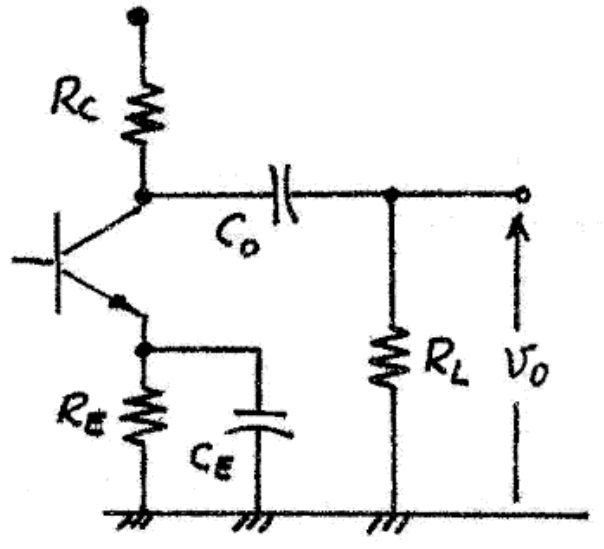
\includegraphics[width=0.4\linewidth]{_fig/multietapas_etapa-salida.png}
	\caption{Circuito de etapa de salida con condensador de acople}
	\label{fig:multietapas_etapa-salida}
\end{figure}

Para el amplificador de continua, queda por obtener una configuración de acoplamiento directo para la etapa de salida.

Una configuración muy buena y popular para la salida que permite acoplamiento directo a la carga es la de simetría complementaria que se muestra en la Figura \ref{fig:multietapas_etapa-salida_simetria-complementaria}. El nivel de continua de la salida es \( 0 \), y la resistencia de salida, \( R_o \), es pequeña. El transistor NPN de arriba conduce para \( V_i \) positivo, y el transistor PNP de abajo conduce para \( V_i \) negativo.

\begin{figure}[h]
	\centering
	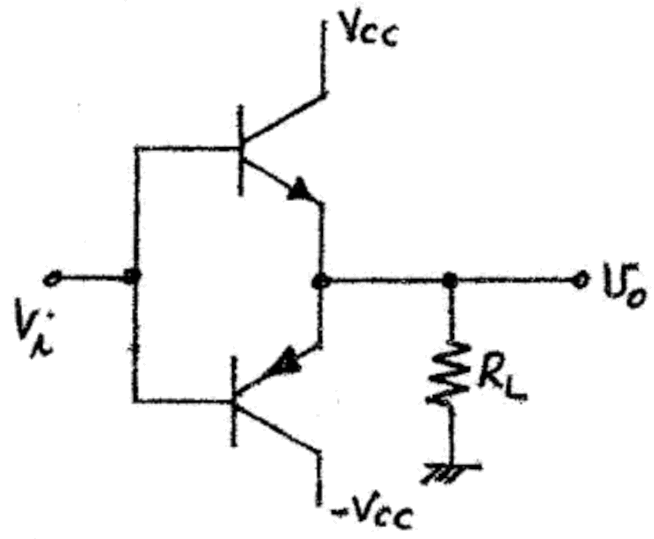
\includegraphics[width=0.4\linewidth]{_fig/multietapas_etapa-salida_simetria-complementaria.png}
	\caption{Circuito de etapa de salida con simetria complementaria}
	\label{fig:multietapas_etapa-salida_simetria-complementaria}
\end{figure}

La configuración tiene el defecto de que \( V_i \) tiene que superar el nivel umbral de tensión en las juntas pn antes de que el transistor correspondiente pueda conducir. La característica de transferencia se muestra en la Figura \ref{fig:multietapas_etapa-salida_característica-transferencia}, donde \( V_\gamma = 0.6 \) para silicio y \( V_\gamma = 0.2 \) para germanio.

\begin{figure}[h]
	\centering
	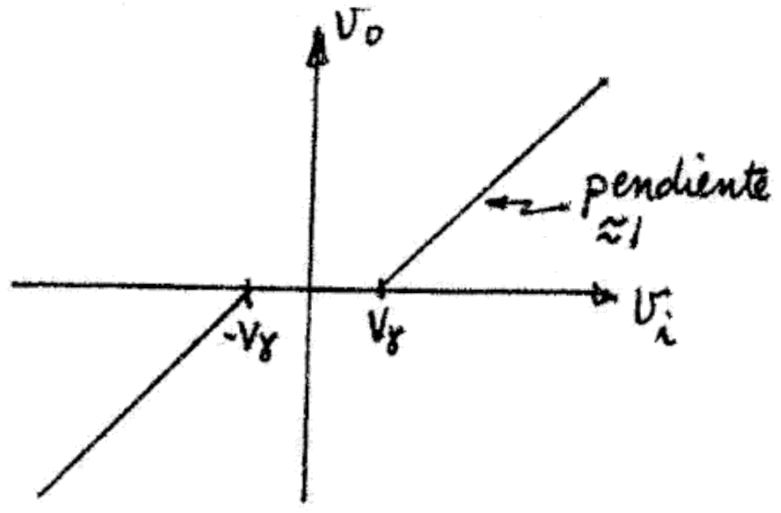
\includegraphics[width=0.4\linewidth]{_fig/multietapas_etapa-salida_característica-transferencia.png}
	\caption{Característica de Transferencia}
	\label{fig:multietapas_etapa-salida_característica-transferencia}
\end{figure}

Esto se puede superar con un esquema de polarizar los transistores al borde de corte, o en la región activa, Figura \ref{fig:multietapas_etapa-salida_polarizacion-diodos} y \ref{fig:multietapas_etapa-salida_polarizacion-resistor}, o utilizar un esquema de retroalimentación para eliminar la distorsión, la Figura \ref{fig:multietapas_etapa-salida_polarizacion-retro}. En los circuitos de la Figura \ref{fig:multietapas_etapa-salida_polarizacion-diodos}, los diodos son polarizados en conducción por las resistencias de base, \( R_B \), de modo que al subir el nivel de entrada sube la señal de base del transistor y varia proporcionalmente la señal de salida.

\begin{figure}[h]
	\centering
	\subfloat[Polarización con diodos]
	{
		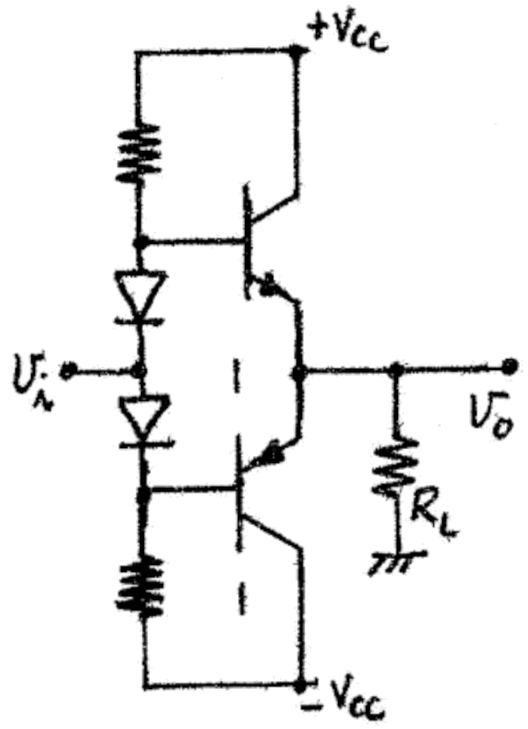
\includegraphics[width=0.28\linewidth]{_fig/multietapas_etapa-salida_polarizacion-diodos.png}
		\label{fig:multietapas_etapa-salida_polarizacion-diodos}
	}
	\subfloat[Con resistencias]
	{
		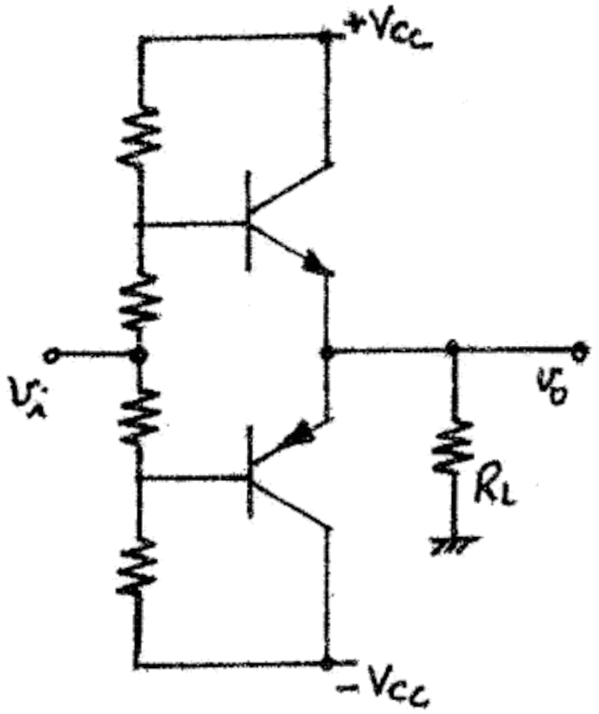
\includegraphics[width=0.28\linewidth]{_fig/multietapas_etapa-salida_polarizacion-resistor.png}
		\label{fig:multietapas_etapa-salida_polarizacion-resistor}
	}
	\subfloat[Uso de retroalimentación]
	{
		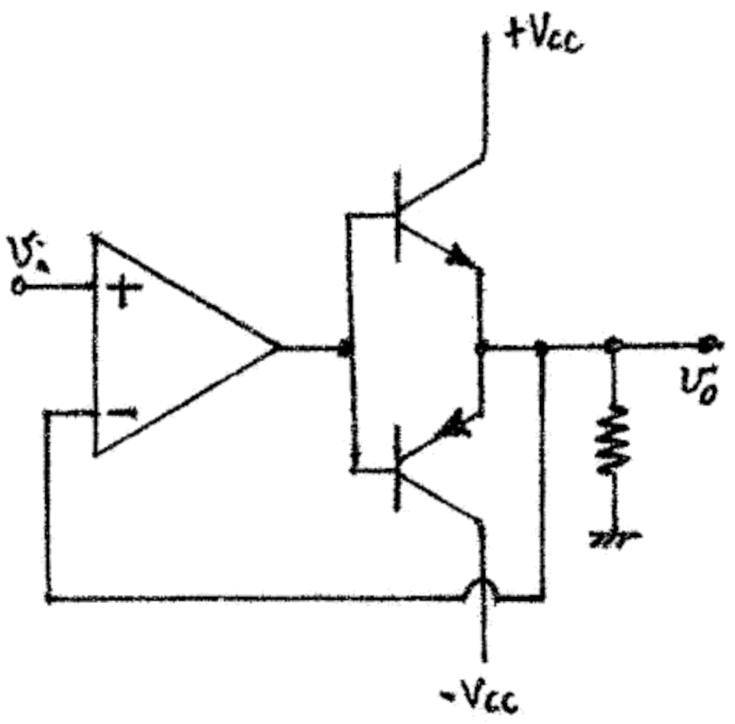
\includegraphics[width=0.38\linewidth]{_fig/multietapas_etapa-salida_polarizacion-retro.png}
		\label{fig:multietapas_etapa-salida_polarizacion-retro}
	}
	\caption{Polarización de Transistores}
	\label{fig:multietapas_etapa-salida_polarizacion}
\end{figure}

\subsection{Estructura interna de circuitos integrados} %109

En esta sección se analizará tres amplificadores construídos como circuitos integrados, el uA730, uA702 y el uA741, de diferentes grados de complejidad y sofisticación.

\subsubsection{El A730}

En la Figura \ref{fig:multietapas_estructura-interna-ic_a730}, se muestra la estructura interna de un circuito integrado sencillo, el A730, y a continuación las características principales dadas por el fabricante.

\begin{figure}[h]
	\centering
	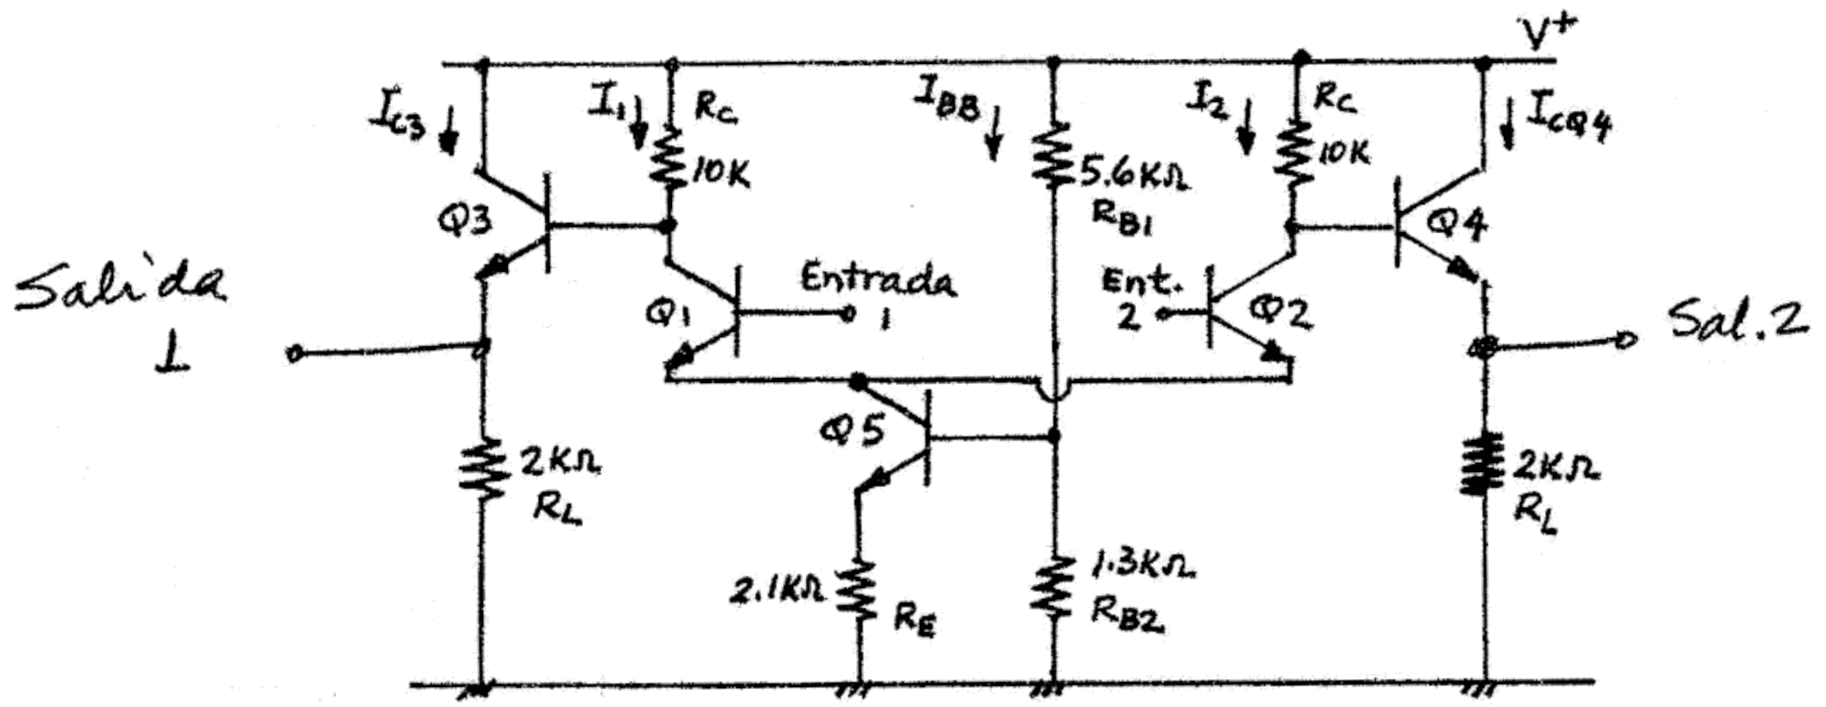
\includegraphics[width=0.8\linewidth]{_fig/multietapas_estructura-interna-ic_a730.png}
	\caption{Estructura interna del A730}
	\label{fig:multietapas_estructura-interna-ic_a730}
\end{figure}

\begin{itemize}
	\item Offset Voltaje: \( 1 \text{mV (max)} \)
	\item Offset Corriente: \( 0.5 \mu \text{A (max)} \)
	\item Corriente de Polarización: \( 3.5 \mu A \)
	\item Rango de Modo Común: \( 2.5 -> 4.5 \)
	\item Rango de Modo Diferencial: \( \pm 5V \)
	\item Ganancia de voltaje: \( 100 \)
	\item Ancho de banda: \( 1.5 \text{MHz} \)
	\item Voltage de suministro: \( 6V < V+ < 14V \), \( V+(tip)=12V \)
	\item CMRR = \( 85 dB \)
	\item Ri = \( 5K\Omega a 20K\Omega \)
\end{itemize}

Se hace notar que el circuito tiene una entrada diferencial y además una salida diferencial, cuyo símbolo se muestra en la Figura \ref{fig:multietapas_estructura-interna-ic_a730-simbolo}. En el circuito, $Q_5$ trabaja como una fuente de corriente, que polariza al par diferencial $Q_1$-$Q_2$, que a su vez impulsan el par diferencial $Q_3$-$Q_4$.

\begin{figure}[h]
	\centering
	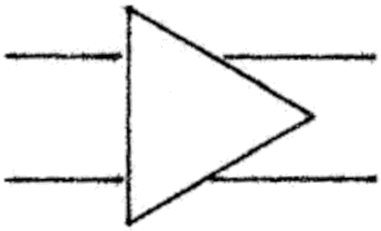
\includegraphics[width=0.3\linewidth]{_fig/multietapas_estructura-interna-ic_a730-simbolo.png}
	\caption{Estructura interna del A730}
	\label{fig:multietapas_estructura-interna-ic_a730-simbolo}
\end{figure}

Con \( V^+ = 12V \) y \( h_{fe} = 150 \), en la base de \( Q_5 \) queda el circuito planteado en la Figura \ref{fig:multietapas_estructura-interna-ic_a730} con su equivalencia de Thevenin, donde \( I_{B5} = 5.26\mu A \) e \( I = 798\mu A \). En equilibrio las corrientes de colector de \( Q_1 \) y \( Q_2 \) son iguales con valor igual a la mitad de \( I \), es decir \( 395\mu A \); por lo tanto se determina una caída en la resistencia de \( 10K\Omega \) de \( 3.95 V \). La corriente de base de estos transistores será: \( \frac{395\mu A}{150} = 2.63\mu A \), y está dentro del límite de \( 3.5\mu A \) máximo especificado por el fabricante. La caída máxima en \( R_C = 10K\Omega \) será \( 7.9V \).

Un extremo del \textbf{rango de modo común} viene dado por la exigencia de que la fuente de corriente permanezca en la región activa. Si el nivel de modo común de las entradas es muy bajo, el transistor \( Q_5 \) saldrá de la región activa (ver Figura \ref{fig:multietapas_estructura-interna-ic_a730-calculo-i}). El nivel mínimo ocurre para el voltaje colector-emisor de \( Q_5 \) apenas superior a saturación, y nos surge la siguiente ecuación:

\begin{figure}[h]
	\centering
	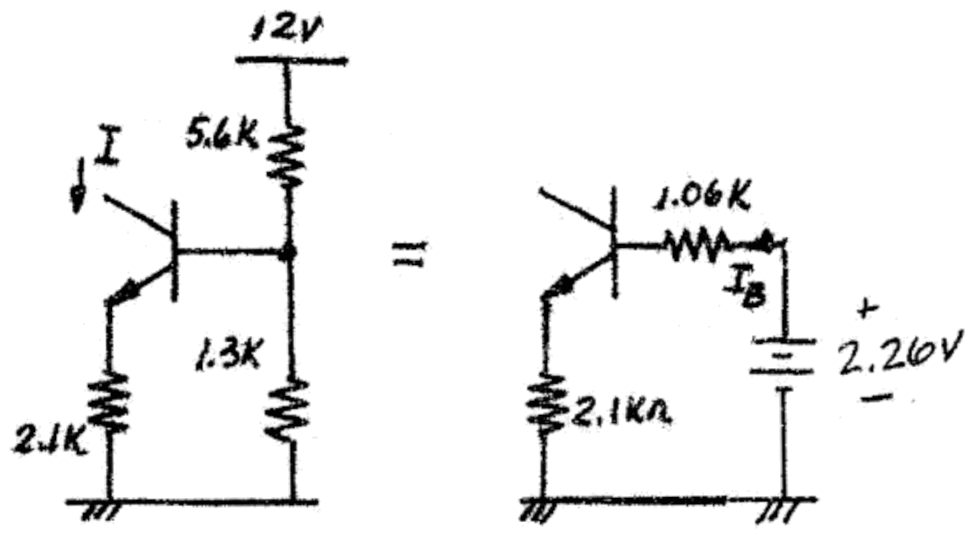
\includegraphics[width=0.3\linewidth]{_fig/multietapas_estructura-interna-ic_a730-calculo-i.png}
	\caption{Calculo del valor de corriente de la fuente de corriente}
	\label{fig:multietapas_estructura-interna-ic_a730-calculo-i}
\end{figure}

\[
V_{A(min)} \geq V_{BE R1} + V_{CE5 (sat)} + V_{E5} = 0.65 + 0.2 + 1.66 = 2.51V
\]

El nivel de modo común máximo viene limitado por la exigencia de que los transistores \( Q_1 \) y \( Q_2 \) admitan las máximas variaciones de la señal de colector sin salir de la región activa. Por lo tanto, surge la siguiente ecuación:

\[
V^+ - I_C R_C - \Delta V_{MAX} - V_{CE(sat)} + 0.6 = 12 - 3.95V - 3.95V - 0.2 + 0.6 = 4.5V
\]

La ganancia de voltaje diferencial a una salida sencilla viene dada por:

\[
G_v = -\frac{\beta R_C}{2r_\pi} \approx -76
\]

Para un amplificador diferencial, la resistencia de entrada viene dada por \( R_i = 2 r_{\pi} \); en este caso

\[
R_i = 2 (r_b + r_{\pi}) = 2 (r_b + 150 V_T / I_C)
\]

\[
R_i = 2 (r_b + 150 \times 26mV / 0.395mA) \approx 20K\Omega
\]

la resistencia de salida viene dada por:

\[
R_o = R_L // \left( \frac{R_C + r_{\pi}}{\beta + 1} \right) \approx 2K // \frac{10K + 10K}{151} \approx 125\Omega
\]

Podemos estimar la corriente total entregada por la fuente de poder, y por lo tanto la potencia disipada bajo condiciones de reposo. La corriente total entregada al circuito de la fuente de poder es:

\[
I_{CC} = I_C3 + I_1 + I_{BQ5} + I_2 + I_{CQ4} = 2(I_C3 + I_1) + I_{B5}
\]

donde: \( I_1 = 395\mu A\), \( I_{B5}(nom) = \frac{12V}{7.9V} = 1.5mA \), \( I_{C3} = \frac{(12 - 3.95 - 0.6)}{2K} = 3.73mA \) 

luego, \( I_{CC} = 12mA \) y la potencia nominal disipada: \( P_{MAX} = 12mA \times 12V = 144mW \)

\subsubsection{El uA702}

A continuación se trata la estructura interna del uA702 y sus características eléctricas principales (ver Figura \ref{fig:multietapas_estructura-interna-ic_ua702}).

\begin{figure}[h]
	\centering
	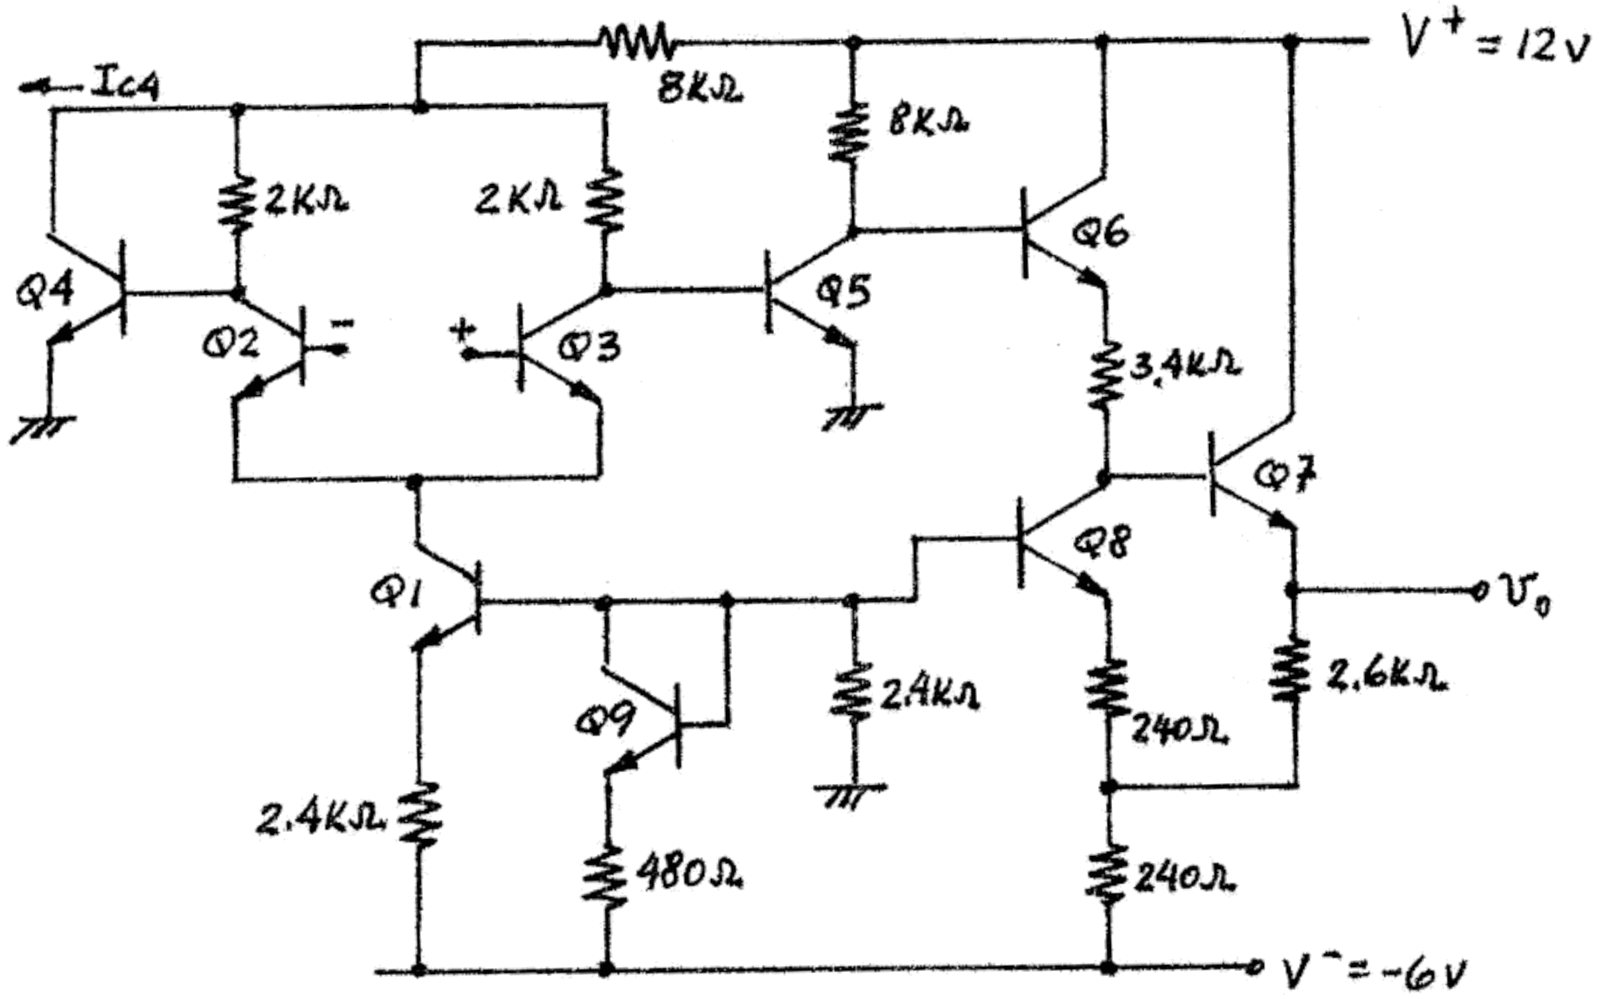
\includegraphics[width=0.8\linewidth]{_fig/multietapas_estructura-interna-ic_ua702.png}
	\caption{Estructura interna del uA702}
	\label{fig:multietapas_estructura-interna-ic_ua702}
\end{figure}

Caracteristicas Eléctricas: ( \( T_A = 25\circ C \), \( V^+ = 12V \), \( V^- = -6V \) )

\begin{table}[h]
	\centering
	\begin{tabular}{|l|c|c|c|c|c|}
		\hline
		\textbf{Parámetros} & \textbf{Condiciones} & \textbf{Min} & \textbf{Típico} & \textbf{Max} & \textbf{Unidad} \\
		\hline
		Voltaje Offset & $R_s < 2K\Omega$ & & 0.5 & 2 & mV \\
		Corriente Offset & & & 180 & 500 & nA \\
		Corr. Polarización & & & 2 & 5 & $\mu$A \\
		$R_{Entrada}$ &  & 16 & 40 &  & K$\Omega$ \\
		Rango Volt. In &  & -4 & & 0.5 & V \\
		CMRR & $R_s < 12K\Omega, F<1KHz$ & 80 & 100 & & dB \\
		Ganancia & $R_L \geq 100K\Omega, V_o = \pm5V$ & 2500 & 3600 & 6000 &  \\
		$R_{Salida}$ &  & 200 & 500 & & $\Omega$ \\
		Corriente Fuente & $V_o = 0$ & & 5.0 & 6.7 & mA \\
		Disipación Potencia & $V_o = 0$ & & 90 & 120 & mW \\
		\hline
	\end{tabular}
	\caption{Características Eléctricas}
\end{table}

El análisis se inicia con los niveles de señal en la condición de reposo.

La corriente que circula por las resistencias de base de Q9 es \( 1.88 mA \), el voltaje en la base de Q1 es \( -4.5V \) (la función de Q9 es la de compensar térmicamente el $V_{BE}$ de Q1); el voltaje a través de la resistencia de emisor de Q1 es \( 0.6V \), lo cual da una corriente de \( 375 \mu A \). 

Bajo condiciones de equilibrio, la corriente de colector de Q2 y Q3 es \( 188 \mu A \). La corriente por la resistencia de 8K es \( 375 \mu A + I_{C4} \) y el voltaje en el colector de Q3 es \( V_{BEQ5} \) es decir \( 0.6 V \). Entonces:

\[
(375\mu A + I_{C4}) \cdot 8K = 12 - (188\mu A) \cdot 2K - 0.6V
\]

de donde, \( I_{C4} = 1mA \). Dado que Q5 tiene un circuito de polarización idéntico a Q4, la corriente de colector de Q5 es igual a la corriente de colector de Q4, o sea \( I_{C5} = I_{C4} = 1mA \). Entonces, \( V_{CEQ5} = 12 - 8 \times 1mA = 4V \).

Para determinar los valores restantes se plantean las siguientes ecuaciones:

\begin{equation}
	I_{C8} \times 3.4K + V_{BEQ7} + I_{C7} \times 248 + (I_{C8} + I_{C7}) \times 248 - 6V = 3.4V
\end{equation}

\begin{equation}
	I_{C8} \times 3.4K + 0.6V + I_{C7} \times 2.6K + (I_{C8} + I_{C7}) \times 248 - 6V = 3.4V
\end{equation}

\begin{equation}
	I_{C8} \times 248 + (I_{C8} + I_{C7}) \times 248 - 6 = -4.5 - 0.6
\end{equation}

Despejando queda \( I_{C7} = 1.9mA \), \( I_{C8} = 920\mu A \) y \( V_o \approx 0.3V \).

Se hace notar que el voltaje de salida es casi \( 0 \); probablemente, si se hace el cálculo con otro valor de \( V_{BE} \), \( V_o \) se aproxima a \( 0V \).

El circuito formado por Q6, Q7 y Q8 es una configuración especial que suministra una ganancia de voltaje, una alta impedancia de entrada y una variación pico a pico del voltaje de salida que es casi igual a la diferencia entre los niveles de las fuentes de poder.

En la Figura \ref{fig:multietapas_estructura-interna-ic_ua702-conf-basica}, se traza la configuración básica:

\begin{figure}[h]
	\centering
	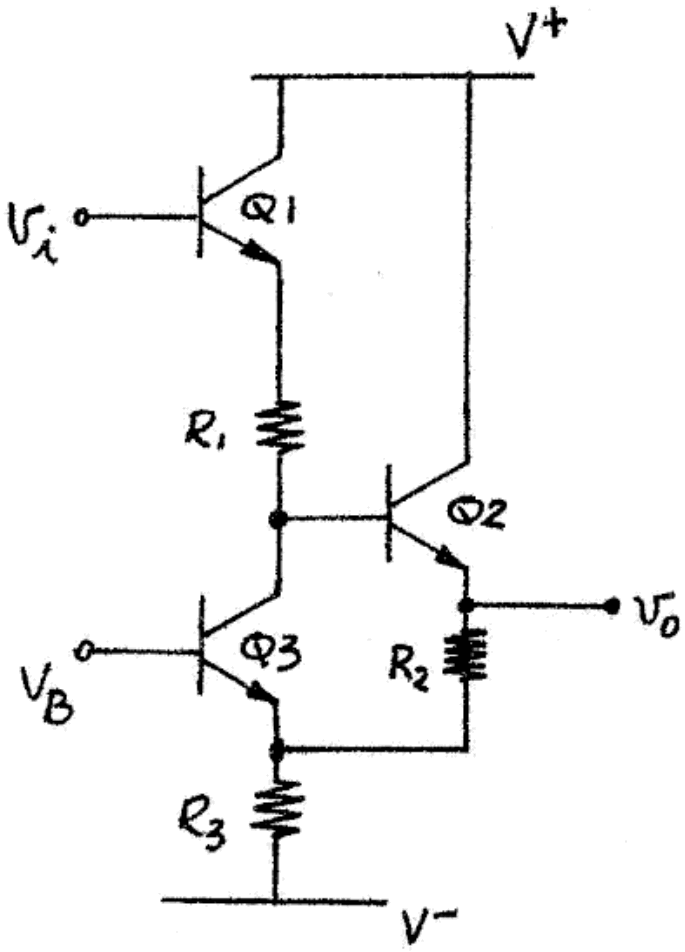
\includegraphics[width=0.4\linewidth]{_fig/multietapas_estructura-interna-ic_ua702-conf-basica.png}
	\caption{Configuración básica}
	\label{fig:multietapas_estructura-interna-ic_ua702-conf-basica}
\end{figure}

Del circuito se tiene que:

\[
V_i = V_{BE1} + I_{C3} R_1 + V_{BE2} + V_o
\]

y para pequeñas variaciones:

\[
V_i + \Delta V_i = V_{BE1} + (I_{C3} + \Delta I_{C3}) R_1 + V_{BE2} + V_o + \Delta V_o
\]

de donde: \( \Delta V_i = \Delta I_{C3} R_1 + \Delta V_o \)

además,

\[
V_B = V_{BE3} + (I_{C3} + \Delta I_{C3} + I_{C2} + \Delta I_{C2}) R_3 - 6
\]

es decir, \( \Delta I_{C3} = -\Delta I_{C2} \)

también, \( \Delta V_o = \Delta I_{C2} R_2 = -\Delta I_{C3} R_2 \Rightarrow \Delta I_{C3} = -\frac{\Delta V_o}{R_2} \)

entonces, \( \Delta V_i = \Delta V_o \left(1 - \frac{R_1}{R_2} \right) \)

y la ganancia, \( \frac{\Delta V_o}{\Delta V_i} = \frac{1}{1 - R_1/R_2} \)

Aplicado al circuito de salida del uA702 se consigue:

\( \Delta V_i = \Delta I_{C8} \times 3.4K + \Delta V_o \)

\( V_B = V_{BE3} + I_{C8} \times 248 + (I_{C8} + I_{C7}) \times 248 \)

\( \Delta I_{C8} = -\frac{\Delta I_{C2}}{2} \)

y, \( \Delta V_{in} = \Delta V_o \left(1 - \frac{3.4K}{5.48K} \right) \)

o

\begin{equation}
	\frac{\Delta V_o}{\Delta V_i} = 2.63
\end{equation}

\subsubsection{El uA741}

A continuación, en la Figura \ref{fig:multietapas_estructura-interna-ic_ua741}, se muestra el uA741, de uso muy extenso, que, a diferencia del uA739 y uA702, ha mantenido su popularidad durante muchos años.

\begin{figure}[h]
	\centering
	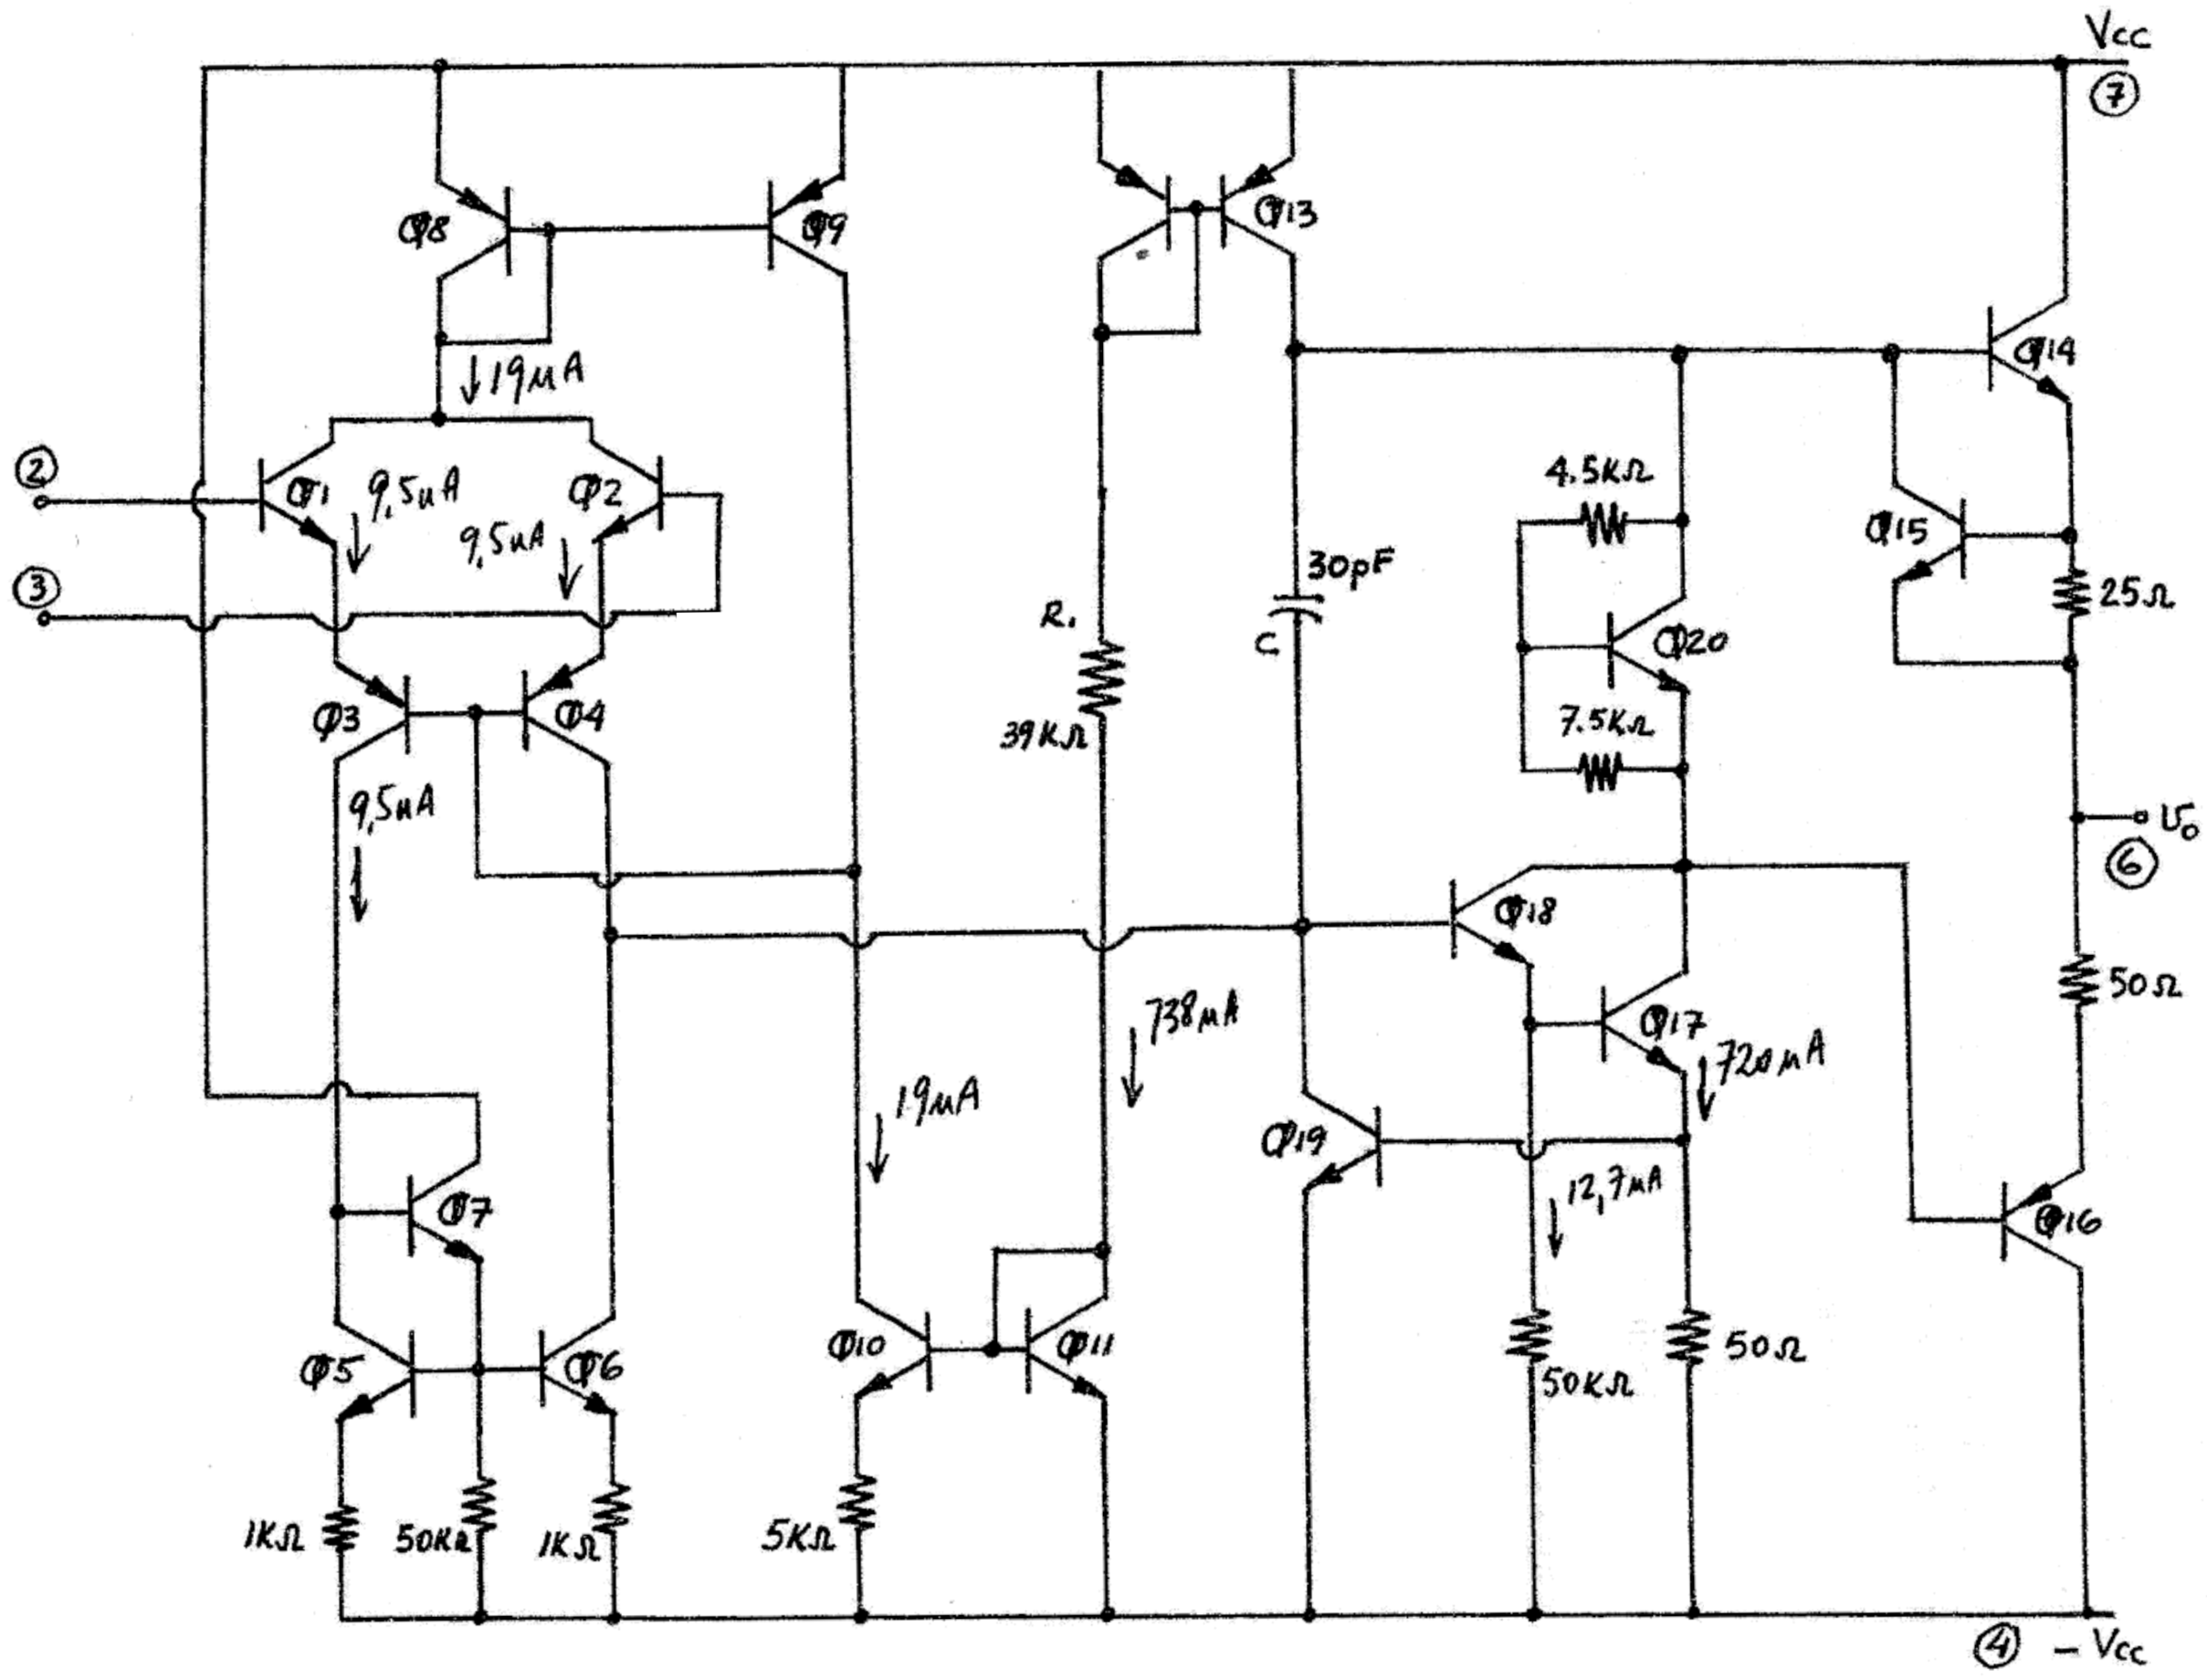
\includegraphics[width=0.8\linewidth]{_fig/multietapas_estructura-interna-ic_ua741.png}
	\caption{Estructura interna del uA702}
	\label{fig:multietapas_estructura-interna-ic_ua741}
\end{figure}

Sus mayores atractivos radican en el amplio rango de variación de los voltajes de entrada y salida, las protecciones y la compensación interna. Su mayor limitación es su ancho de banda.

Q1 y Q2 están en colector común, mientras que Q3 y Q4 están en base común. Estos cuatro transistores forman una etapa diferencial Cascode con una CMRR alta, $R_i$ alta y una ganancia diferencial del orden de \( 200 \). Q6 es la carga activa de Q4. Q5 y Q7 intervienen para polarizar Q6. Q10 y Q11 forman una fuente de baja corriente que suministra la corriente de polarización de base de Q3 y Q4 y una $I_C$ fija a Q9. Los transistores Q8 y Q9, junto con Q10 y Q11, fijan las corrientes de polarización para la etapa diferencial, de modo que: \( I_t = I_{C0} + I_{C1} + I_{C2} \). La interconexión de \(Q9\) con \(Q4\) y \(Q3\) en lazo cerrado ayuda a mantener \(I_{C1}\) e \(I_{C2}\) independientes de las variaciones de \(h_{fe}\).

La salida del amplificador diferencial alimenta al par Darlington \(Q18\) y \(Q17\) conectado como emisor común. \(Q13\) actúa tanto como carga activa para el par Darlington y como una fuente de corriente de polarización de \(Q20\) de manera que para señal cero una corriente de \(200\) \(\mu A\) circula por los transistores de salida.	\(Q12\) polariza a \(Q13\) y a través de la resistencia \(R_1\) suministra una corriente constante a \(Q11\). El amplificador Darlington tiene una ganancia de voltaje cercana a \(1000\) y excita a los amplificadores de salida, configurados como seguidores de emisor clase AB, formado por \(Q14\) y \(Q16\). El transistor \(Q20\) trabaja como un diodo Zener para dar la polarización apropiada entre las bases de \(Q14\) y \(Q16\).

Debido al efecto Miller, la capacitancia \(C\) se multiplica por la ganancia del par Darlington y crea así el polo dominante que hace el amplificador operacional estable.

Los transistores \(Q15\) y \(Q19\) forman la protección de cortocircuito. Normalmente están en corte debido a la poca caída de voltaje a través de \(R_2\) y \(R_3\) respectivamente. Cuando aumenta exorbitantemente la corriente por estas resistencias, el aumento en la caída de voltaje a través de ellas enciende a \(Q15\) o \(Q19\), desviando así la señal que impulsa la etapa de salida. La corriente de salida se limita a \( \frac{V_{BE}}{R_2} \), es decir, aproximadamente \( 25 \text{mA} \).

\section{Problemario} %p119
- pendiente en apuntes -